\chapter{Solides et Volumes}\label{ChSolidesVolumes}


\vspace{5cm}
\begin{acquis}
\begin{itemize}
\item Comprendre et utiliser le vocabulaire des solides (sommets, arêtes, faces);
\item représenter un pavé droit en perspective cavalière;
\item construire le patron d’un pavé droit;
\item compléter un patron de prisme droit;
\item de manipuler les unités de volume et les convertir;
\item calculer le volume d’un pavé droit;
\item calculer des volumes de solides constitués de plusieurs pavés droits.
\end{itemize}
\end{acquis}

\activites

\begin{activite}[Un p'tit tour dans l'Espace !]

\begin{partie}[Quelques représentations]
\begin{minipage}[c]{0.19\linewidth}
 \begin{center}  
\includegraphics[width=1.9cm]{espace_obj1} \end{center}
 \end{minipage} \hfill%
\begin{minipage}[c]{0.19\linewidth}
 \begin{center}  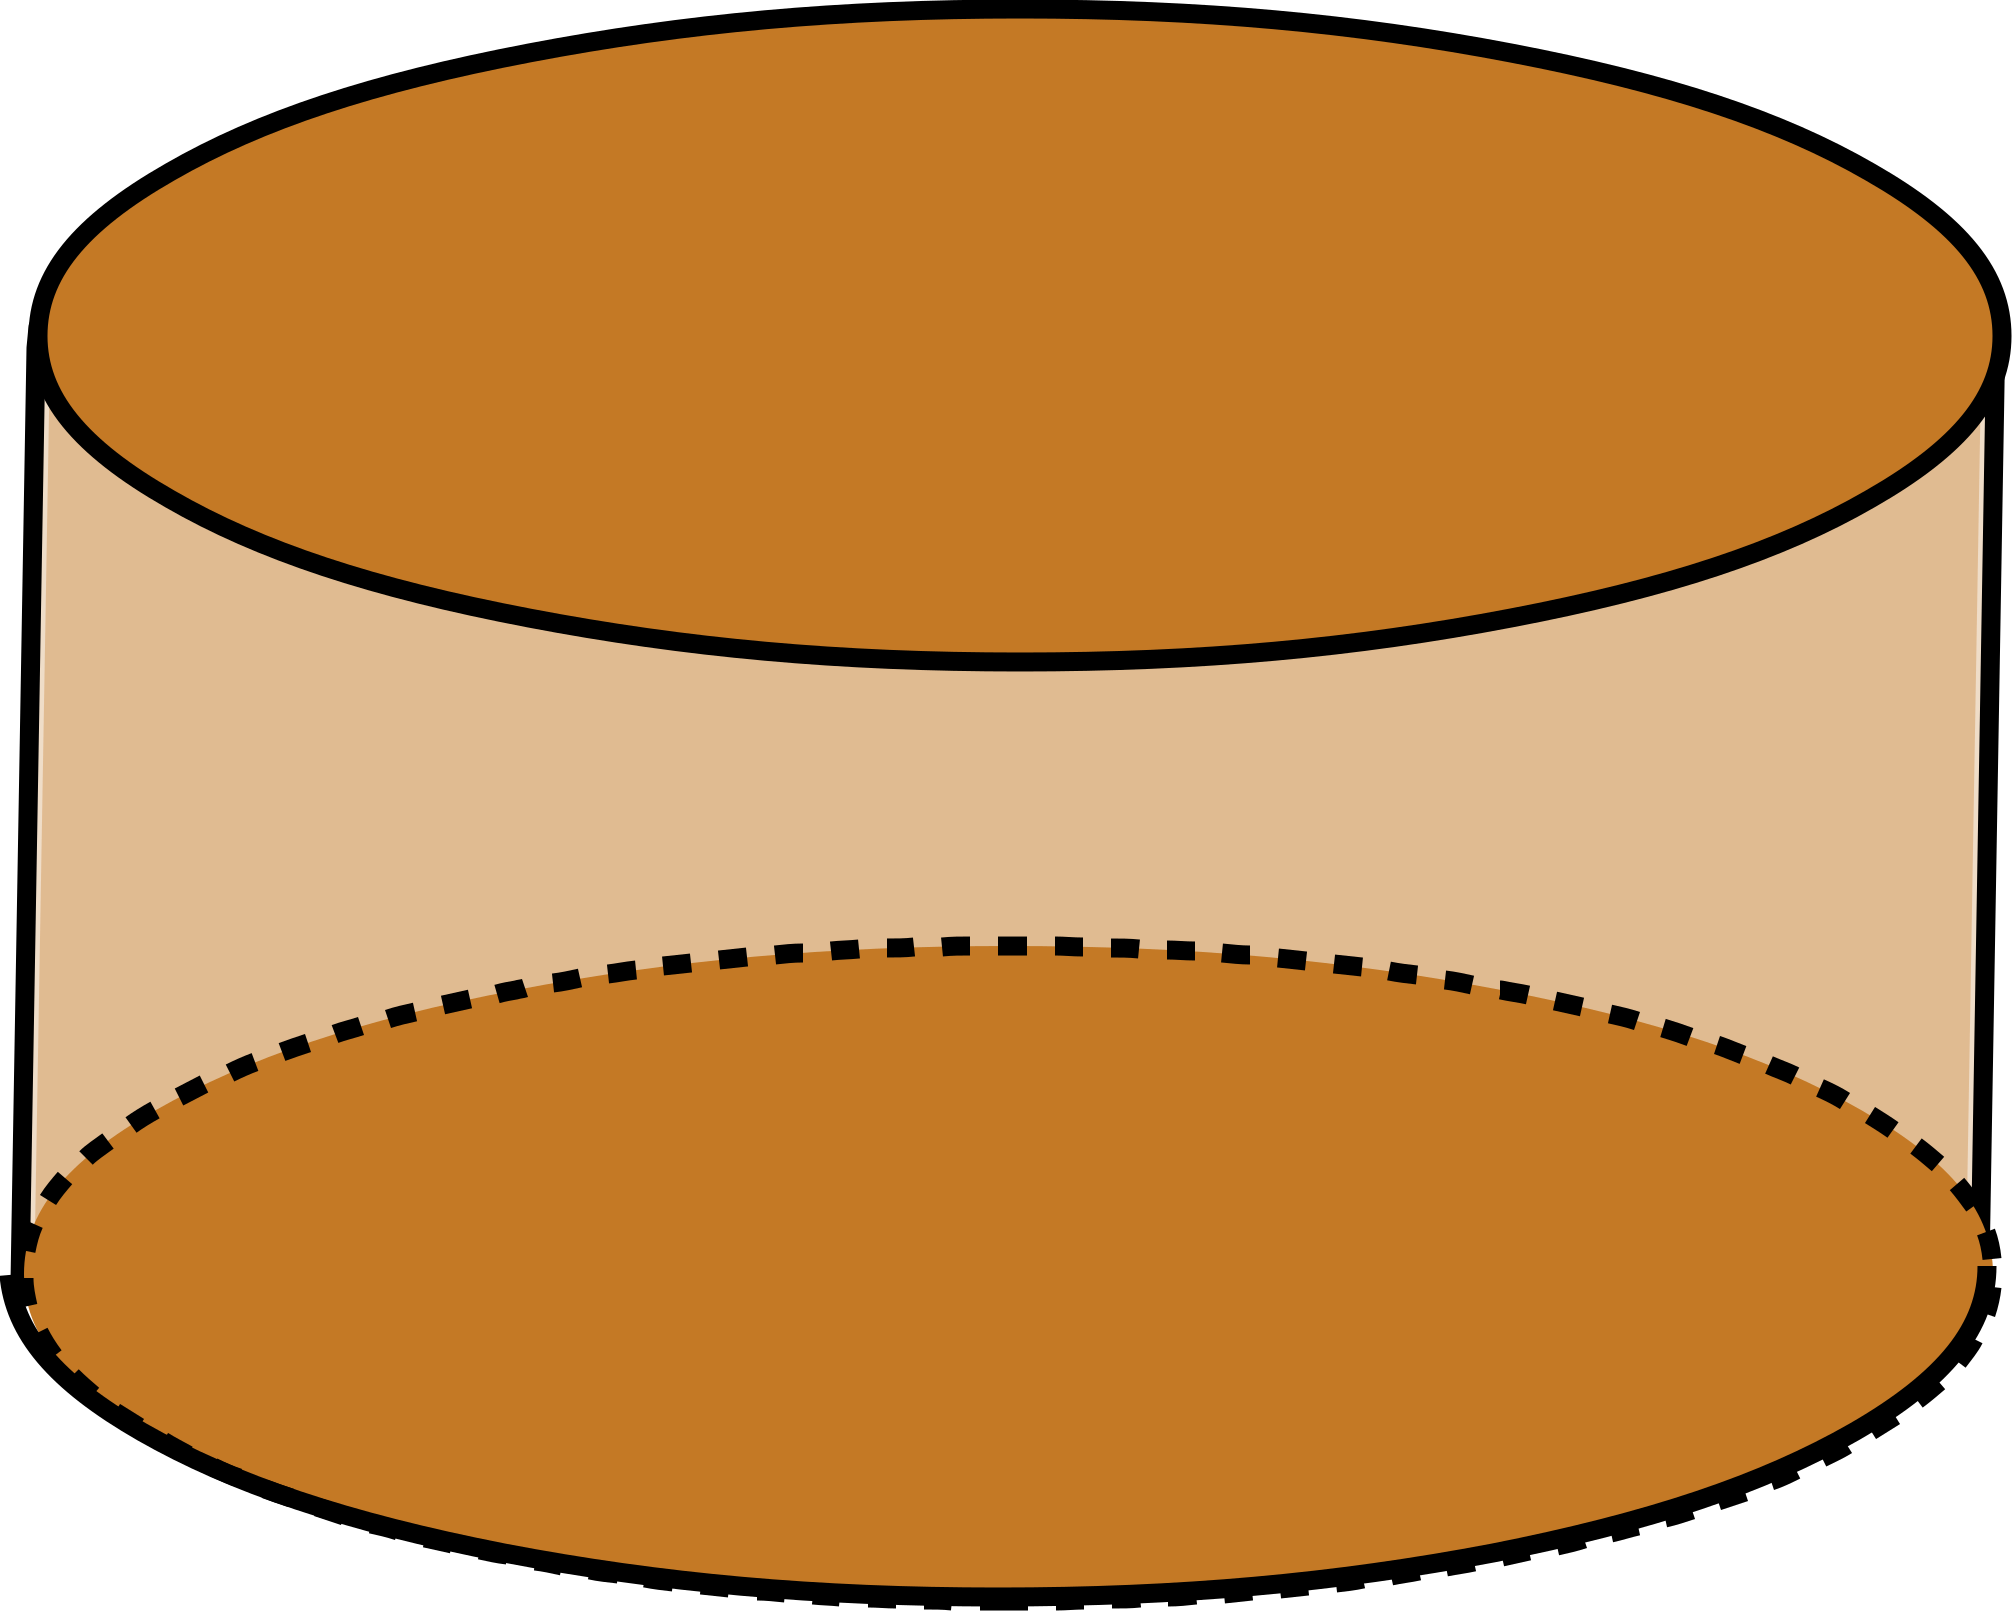
\includegraphics[width=2.1cm]{espace_obj2} \end{center}
 \end{minipage} \hfill%
\begin{minipage}[c]{0.19\linewidth}
 \begin{center}  
\includegraphics[width=1.6cm]{espace_obj3} \end{center}
 \end{minipage} \hfill%
\begin{minipage}[c]{0.19\linewidth}
 \begin{center}  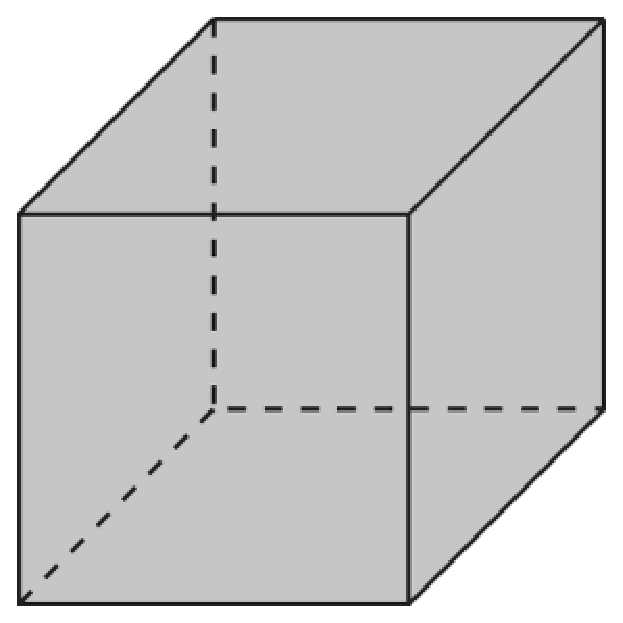
\includegraphics[width=2.1cm]{espace_obj4} \end{center}
 \end{minipage} \hfill%
\begin{minipage}[c]{0.19\linewidth}
 \begin{center}  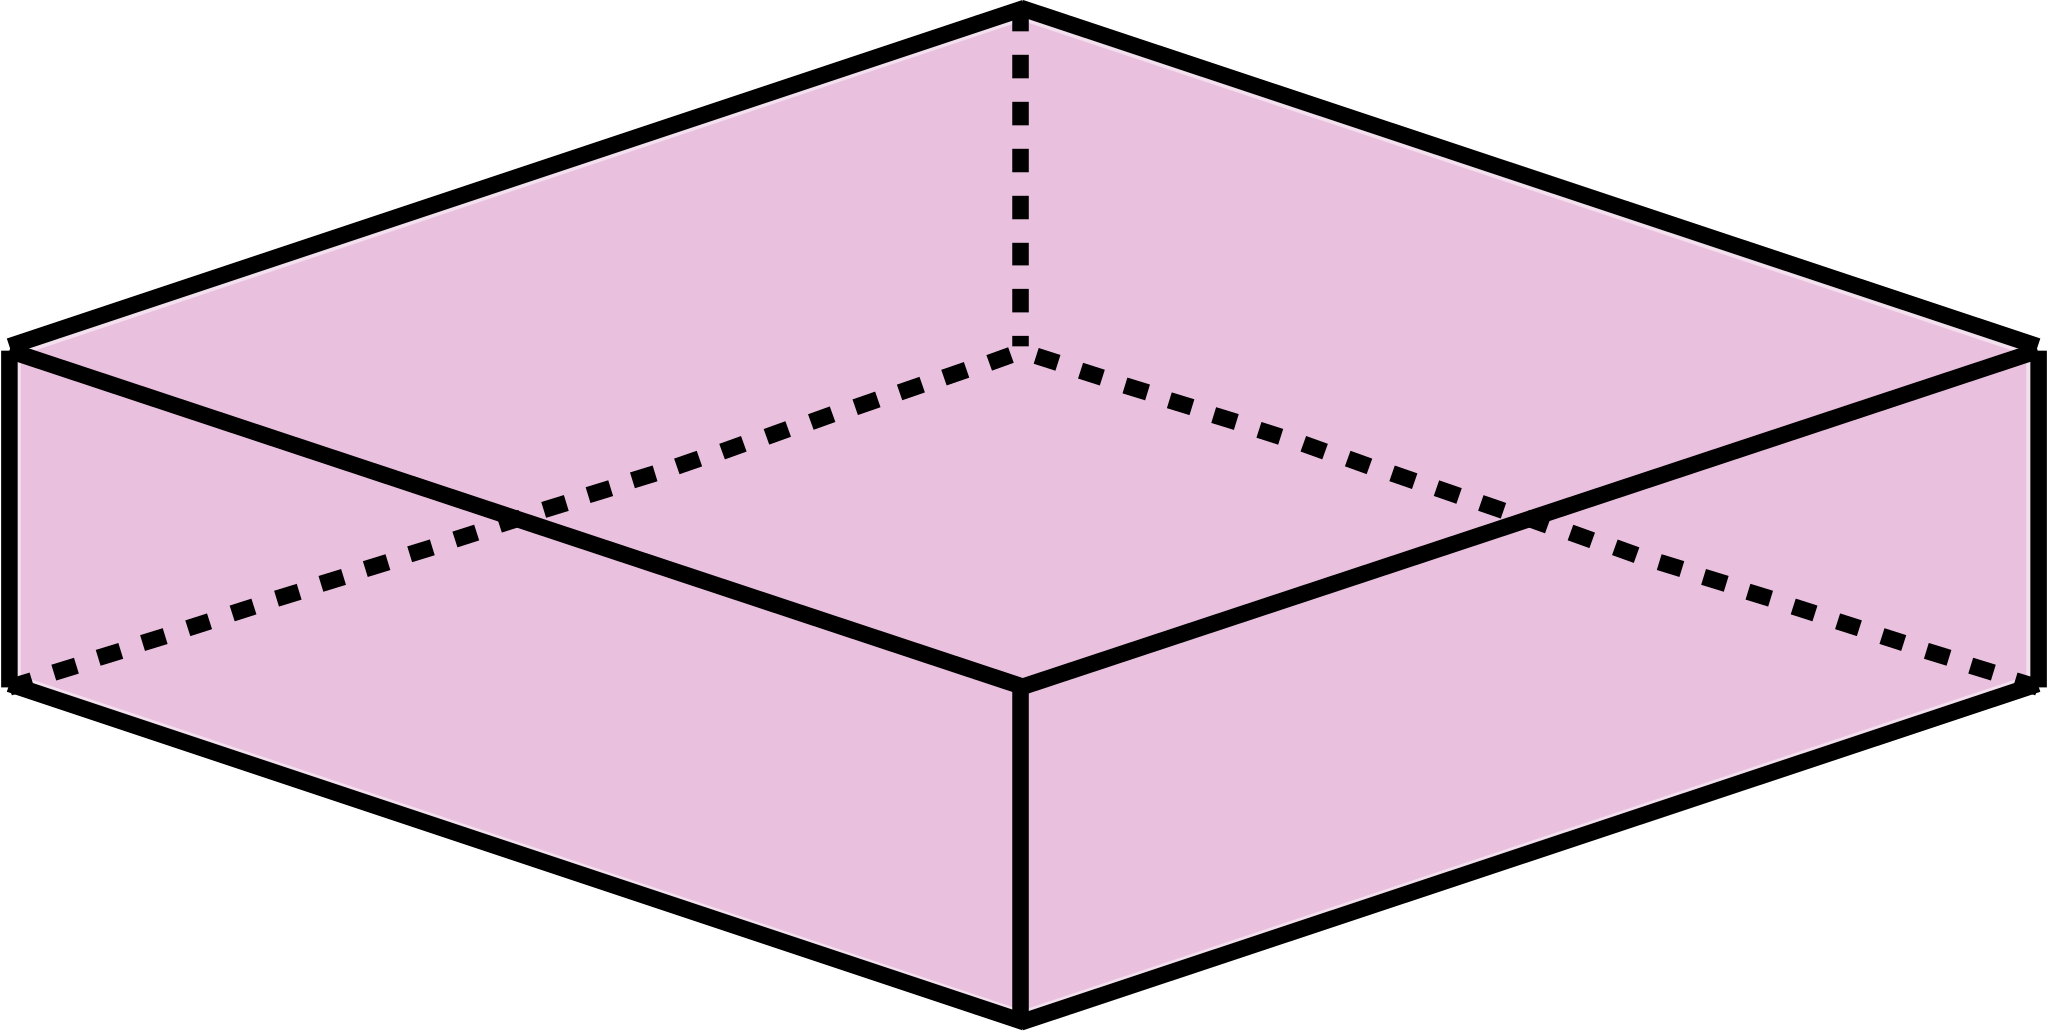
\includegraphics[width=2.5cm]{espace_obj5} \end{center}
 \end{minipage} \\
 
\begin{minipage}[c]{0.19\linewidth}
\begin{center} objet 1 \end{center}
 \end{minipage} \hfill%
\begin{minipage}[c]{0.19\linewidth}
 \begin{center} objet 2 \end{center}
 \end{minipage} \hfill%
\begin{minipage}[c]{0.19\linewidth}
\begin{center} objet 3 \end{center}
 \end{minipage} \hfill%
\begin{minipage}[c]{0.19\linewidth}
\begin{center} objet 4 \end{center}
 \end{minipage} \hfill%
\begin{minipage}[c]{0.19\linewidth}
\begin{center} objet 5 \end{center}
 \end{minipage} \\
\begin{enumerate}
 \item À quels objets de la vie courante te font penser les objets ci‑dessus ?
 \item Pourquoi y a‑t‑il des traits en pointillés ?
 \item Pour les \emph{objets 1}, \emph{4} et \emph{5}, indique le nombre de \textbf{faces}, d'\textbf{arêtes} et de \textbf{sommets}.
 \item Pour chaque objet, dessine à main levée une représentation possible de la vue de dessus.
 \item Dans la réalité, les faces de l'\emph{objet 5} sont des rectangles. Qu'en est‑il dans sa représentation ci‑dessus ?
 \end{enumerate}
\end{partie}

\begin{partie}[Perspective cavalière]
\begin{minipage}[c]{0.58\linewidth}
\begin{enumerate}
 \item Plusieurs perspectives existent. Celle de l'objet 5 est appelée perspective dimétrique. On veut le représenter en \textbf{perspective cavalière} dont une particularité est d'avoir une face en vraie grandeur. On a commencé son tracé. Reproduis‑le et complète‑le en utilisant le quadrillage.
 \item Représente maintenant un cube en perspective cavalière en prenant cinq carreaux pour côté du carré en vraie grandeur. 
 \end{enumerate}
 \end{minipage} \hfill%
 \begin{minipage}[t]{0.38\linewidth}
  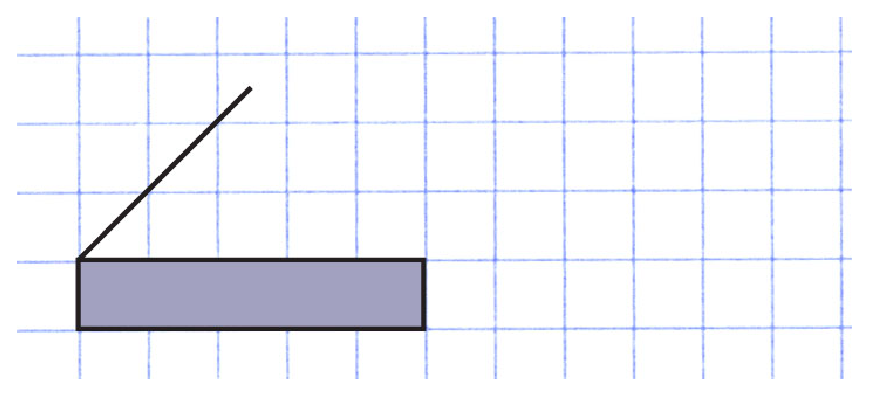
\includegraphics[width=5.5cm]{cavaliere}
  \end{minipage} \\
\end{partie}

\end{activite}

%%%%%%%%%%%%%%%%%%%%%%%%%%%%%%%%%%%%%%%%%%%%%%%%%%%%%%%%%%%%%%%%%%%%%%%%%%

\begin{activite}[De l'enveloppe au cube]

\begin{partie}[Préparation de l'enveloppe]
\begin{enumerate}
 \item Achète une enveloppe standard de format 11 cm × 22 cm et plie‑la en deux de façon à obtenir un carré (figure 1).
 \item Repère le centre d'un carré au crayon (figure 2). 
 \item Ramène les sommets du carré vers le centre en marquant bien les plis des deux côtés (figures 3 et 4). Déplie, tu dois obtenir la figure 5.
 \end{enumerate}
\begin{minipage}[c]{0.21\linewidth}
 \begin{center}  
\includegraphics[width=2.4cm]{enveloppe_c1} \end{center}
 \end{minipage} \hfill%
\begin{minipage}[c]{0.21\linewidth}
 \begin{center}  
\includegraphics[width=2.4cm]{enveloppe_c2} \end{center}
 \end{minipage} \hfill%
\begin{minipage}[c]{0.16\linewidth}
 \begin{center}  
\includegraphics[width=1.2cm]{enveloppe_c3} \end{center}
 \end{minipage} \hfill%
\begin{minipage}[c]{0.16\linewidth}
 \begin{center}  
\includegraphics[width=1.5cm]{enveloppe_c4} \end{center}
 \end{minipage} \hfill%
\begin{minipage}[c]{0.21\linewidth}
 \begin{center}  
\includegraphics[width=2.6cm]{enveloppe_c5} \end{center}
 \end{minipage} \\
 
\begin{minipage}[c]{0.19\linewidth}
\begin{center} figure 1 \end{center}
 \end{minipage} \hfill%
\begin{minipage}[c]{0.19\linewidth}
 \begin{center} \qquad figure 2 \end{center}
 \end{minipage} \hfill%
\begin{minipage}[c]{0.19\linewidth}
\begin{center} \qquad figure 3 \end{center}
 \end{minipage} \hfill%
\begin{minipage}[c]{0.19\linewidth}
\begin{center} figure 4 \end{center}
 \end{minipage} \hfill%
\begin{minipage}[c]{0.19\linewidth}
\begin{center} figure 5 \end{center}
 \end{minipage} \\
\end{partie}

\begin{partie}[Abracadabra !]
Découpe le haut de l'enveloppe pour l'ouvrir (figure 5). En ouvrant l'enveloppe, tu dois voir apparaître un cube !  \\[0.5em]
Colle cette enveloppe dans une double page de ton cahier de façon à ce que le cube se reforme quand tu ouvres ton cahier au niveau de cette double page.
\end{partie}

\end{activite}

%%%%%%%%%%%%%%%%%%%%%%%%%%%%%%%%%%%%%%%%%%%%%%%%%%%%%%%%%%%%%%%%%%%%%%%%%%

\begin{activite}[La chasse aux cubes]

\begin{partie}[Pour commencer \ldots]
\begin{minipage}[c]{0.58\linewidth}
Julien dispose d'un jeu de cubes tels que celui‑ci : 
 \end{minipage} \hfill%
\begin{minipage}[c]{0.38\linewidth}

\includegraphics[width=1.2cm]{chasse_c1}
 \end{minipage} \\
\begin{minipage}[c]{0.7\linewidth}
En assemblant six de ces cubes, il obtient un nouveau solide : 
 \end{minipage} \hfill%
\begin{minipage}[c]{0.26\linewidth}
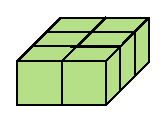
\includegraphics[width=2.2cm]{chasse_c2}
 \end{minipage} \\
\begin{enumerate}
 \item Comment s'appelle ce solide ?
 \item Combien a‑t‑il de faces ? Donne la nature de chaque face. Combien y en a‑t‑il de différentes tailles ? Dessine chacune d'elles en vraie grandeur sachant que l'arête du petit cube est 1 cm.
 \item Dessine ce solide en perspective cavalière et colorie deux de ses faces parallèles. Au total, combien y a‑t‑il de paires de faces parallèles ?
 \end{enumerate}
\end{partie}

\begin{partie}[Un peu plus dur \ldots]
\begin{enumerate}
 \item Avec huit cubes, combien peut‑on construire de \textbf{pavés droits} différents ?
 \item Dessine en perspective cavalière et à main levée tous les solides obtenus. (Tu pourras t'aider de papier pointé.) Est‑ce que certains sont « plus particuliers » que d'autres ?
 \item Quel(s) est (sont) celui (ceux) qui a (ont) la plus grande arête ? La plus petite arête ?
 \item Quel(s) est (sont) celui (ceux) qui a (ont) la plus grande face ? La plus petite face ?
 \item Ont‑ils tous le même nombre de sommets ?
 \end{enumerate}
\end{partie}

\end{activite}

%%%%%%%%%%%%%%%%%%%%%%%%%%%%%%%%%%%%%%%%%%%%%%%%%%%%%%%%%%%%%%%%%%%%%%%%%%

\begin{activite}[Patron du pavé droit]

\begin{partie}[Dimensions de la boîte]
Gilles a sous les yeux une boîte qu'il voudrait reconstruire à l'identique, en papier. Cette boîte a la forme d'un pavé droit. 
\begin{enumerate}
 \item Il mesure les côtés d'une face et trouve 2,5 cm et 3,5 cm. Reproduis cette face en grandeur réelle sur ton cahier.
 \item Il mesure une autre face et constate qu'elle a la même largeur que la première et qu'elle est deux fois plus longue. Reproduis cette seconde face.
 \item Malheureusement, il n'a pas le temps de prendre d'autres mesures et doit rentrer chez lui. Avec ce qu'il a pu mesurer, a‑t‑il toutes les informations pour reconstruire la boîte ? Si oui, donne les dimensions de la troisième face et reproduis-la.
 \end{enumerate}
\end{partie}

\begin{partie}[Vers le patron]
\begin{enumerate}
 \item Construis un \textbf{patron} possible de ce pavé droit. Y a‑t‑il plusieurs possibilités ?
 \item Découpe et assemble le patron.
 \end{enumerate}
\end{partie}

\begin{partie}[Emballer c'est peser]
\begin{minipage}[c]{0.78\linewidth}
 \begin{enumerate}
  \item On utilise du ruban pour ficeler cette boîte. Sachant qu'il en faut 9 cm pour le nœud, quelle est la longueur de ruban nécessaire ?
  \item Il y a deux autres façons de la ficeler. Pour chacune, fais un schéma et calcule la longueur de ruban nécessaire.
  \item Quelle est la méthode qui nécessite le moins de ruban ?
 \end{enumerate}
\end{minipage} \hfill%
\begin{minipage}[c]{0.18\linewidth}
 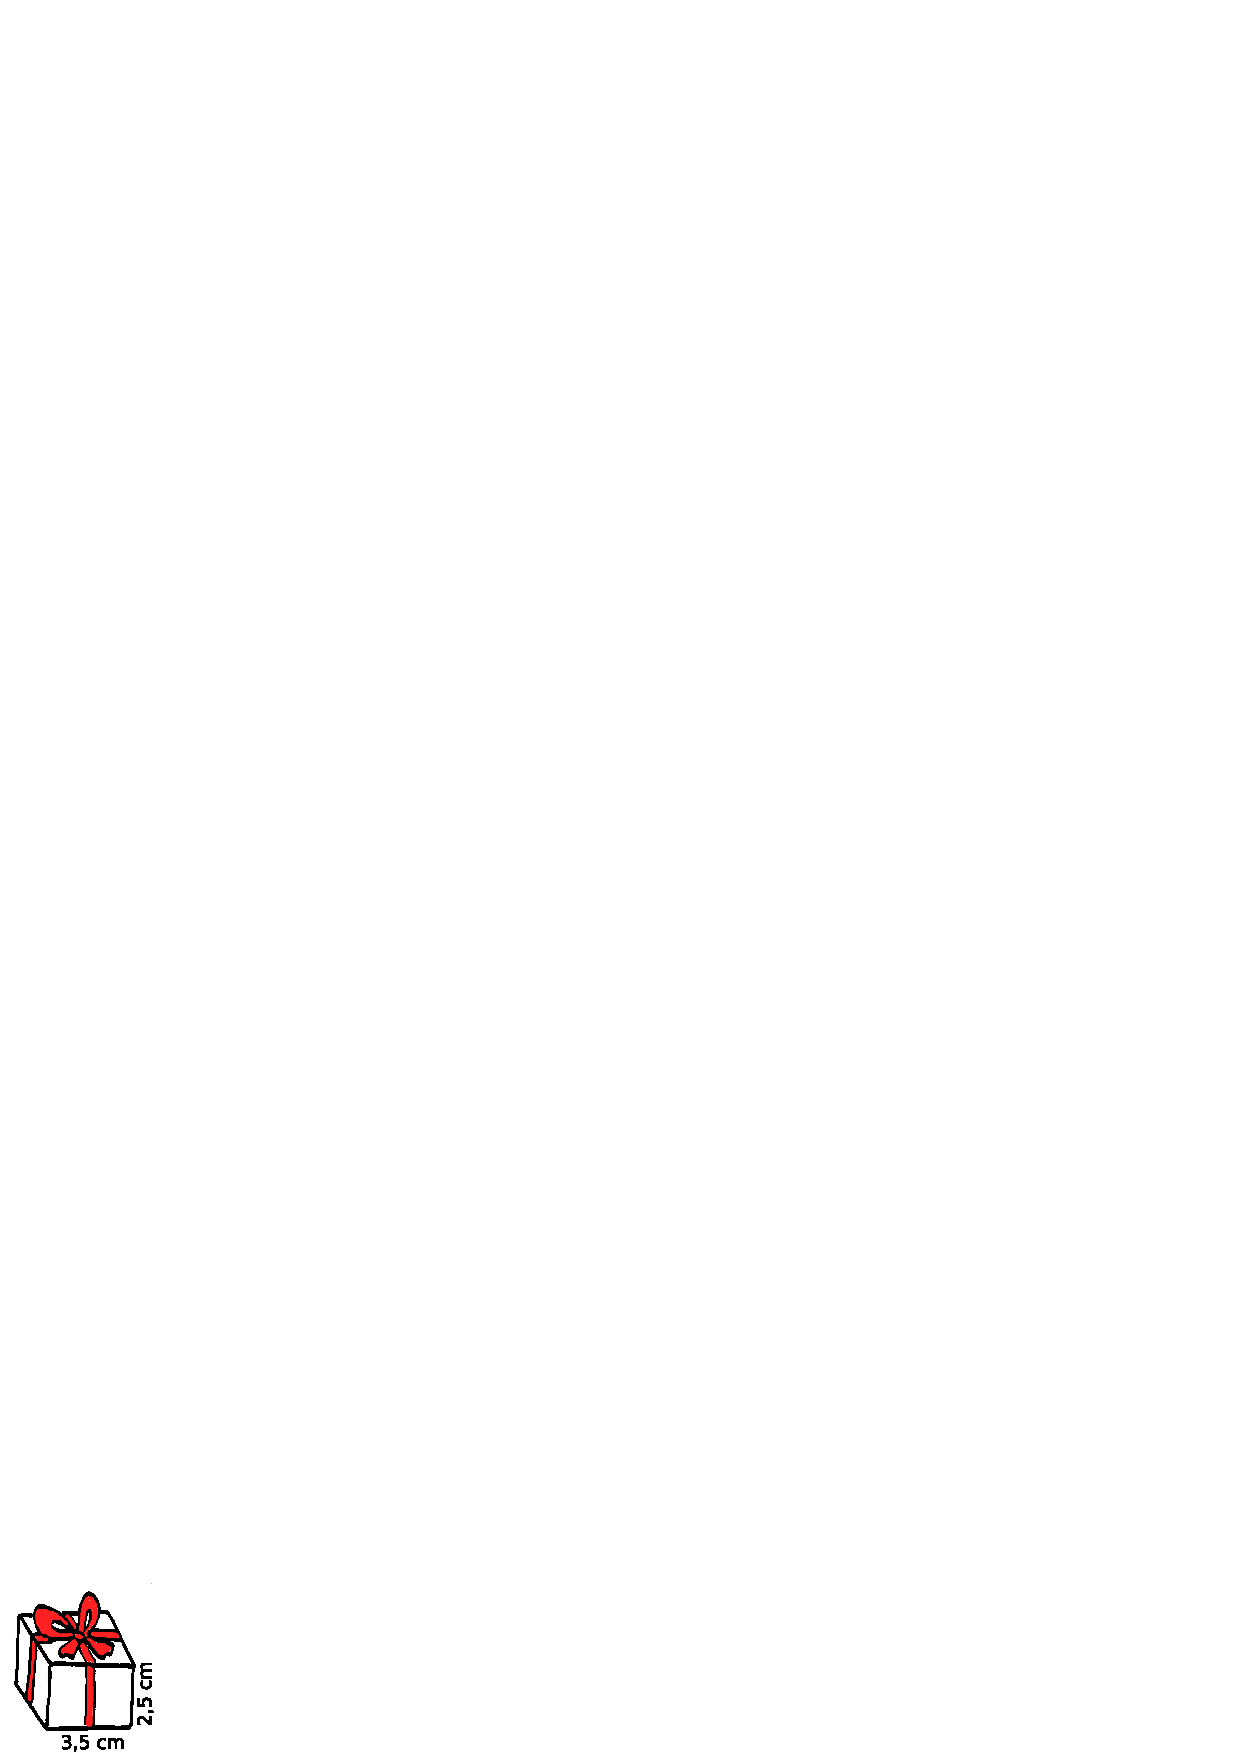
\includegraphics[width=2.5cm]{cadeau_emballage}
\end{minipage} \\
\end{partie}

\end{activite}

%%%%%%%%%%%%%%%%%%%%%%%%%%%%%%%%%%%%%%%%%%%%%%%%%%%%%%%%%%%%%%%%%%%%%%%%%%

\begin{activite}[Volume d'un parallélépipède rectangle]

\begin{partie}
On souhaite remplir la boîte ci-dessous en forme de \textbf{parallélépipède rectangle} avec des cubes d'un centimètre d'arête. On rappelle qu'un cube de 1 cm d'arête a un \textbf{volume} de 1 cm\up{3}. \\[0.5em]
\begin{center}  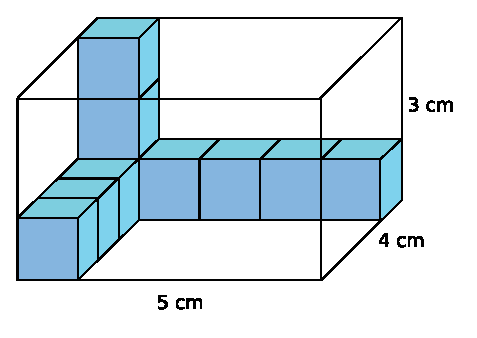
\includegraphics[width=6cm]{boite_remplir} \end{center}
\begin{enumerate}
 \item Combien de cubes faut‑il pour remplir le fond de la boîte ?
 \item En comptant les cubes déjà dans la boîte, combien de couches faut‑il pour remplir toute la boîte ?
 \item En comptant les cubes déjà dans la boîte, combien de cubes faut‑il au total pour remplir toute la boîte ?
 \item Déduis‑en le volume de cette boîte.
 \end{enumerate}
\end{partie}

\begin{partie}
Reprends les questions précédentes avec une boîte de dimensions 9 cm, 10 cm, 12 cm.
\end{partie}

\begin{partie}
Quelles dimensions doit‑on connaître pour calculer le volume d'un parallélépipède rectangle ? Déduis‑en une formule permettant de le calculer.
\end{partie}

\end{activite}

%%%%%%%%%%%%%%%%%%%%%%%%%%%%%%%%%%%%%%%%%%%%%%%%%%%%%%%%%%%%%%%%%%%%%%%%%%

\begin{activite}[Conversions]

\begin{partie}
Un parallélépipède rectangle a pour dimensions 4 cm, 6 cm et 8 cm.
\begin{enumerate}
 \item Quel est son volume en cm\up{3} ?
 \item Combien faut-il de cubes de 1 mm d'arête pour le remplir ?
 \item Quel est son volume en mm\up{3} ?
 \item Quelle opération doit-on effectuer pour passer du volume d'un solide en cm\up{3} à son volume en mm\up{3} ?
 \end{enumerate}
\end{partie}

\vspace{2em}

\begin{minipage}[c]{0.8\linewidth}
\begin{partie}[Une petite expérience]
\begin{enumerate}
 \item Trouve un récipient de forme parallélépipédique. Mesure ses dimensions et calcule son volume en dm\up{3}.
 \item Quelle est la \textbf{capacité} de ce récipient en litres ? (Si elle n'est pas indiquée sur le récipient, tu pourras le remplir d'eau puis mesurer sa capacité à l'aide d'une éprouvette graduée.)
 \item Déduis-en alors la correspondance entre un volume en dm\up{3} et une capacité en litres.
 \end{enumerate}
\end{partie}
 \end{minipage} \hfill%
\begin{minipage}[c]{0.16\linewidth}
 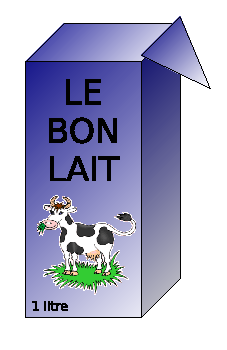
\includegraphics[width=2.5cm]{bon_lait}
\end{minipage} \\

\end{activite}

%%%%%%%%%%%%%%%%%%%%%%%%%%%%%%%%%%%%%%%%%%%%%%%%%%%%%%%%%%%%%%%%%%%%%%%%%%


\cours
%\section{Une section}

% remarque : pour qu'un mot se retrouve dans le lexique : \MotDefinition{asymptote horizontale}{} 

\begin{aconnaitre}
Lorsqu'on représente un solide en \MotDefinition{perspective cavalière}{} :
\begin{itemize}
 \item La face avant est représentée en vraie grandeur ;
 \item Les arêtes parallèles sont représentées par des segments parallèles ;
 \item Les arêtes cachées sont dessinées en pointillés.
 \end{itemize}
\end{aconnaitre}

\begin{methode*1}[Représenter en perspective cavalière]

 \begin{exemple*1}
 
 \begin{minipage}[c]{0.62\linewidth}
 Complète la représentation en perspective cavalière du pavé droit ci‑contre.
  \end{minipage} \hfill%
  \begin{minipage}[c]{0.32\linewidth} 
   
\includegraphics[width=3cm]{persp_xyz}
   \end{minipage} \\[1.4em]
   
 \begin{minipage}[t]{0.32\linewidth}   
On commence par la face avant, en vraie grandeur.
  \end{minipage} \hfill%
  \begin{minipage}[t]{0.32\linewidth}
On trace les arêtes transversales, parallèles et de même longueur, mais pas en vraie grandeur.
  \end{minipage} \hfill%
   \begin{minipage}[t]{0.32\linewidth}   
On finit par la face arrière, en vraie grandeur.
   \end{minipage} \\
   
 \begin{minipage}[c]{0.3\linewidth}     
\begin{center} 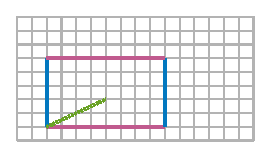
\includegraphics[width=3cm]{persp_rectangle1} \end{center}
  \end{minipage} \hfill%
  \begin{minipage}[c]{0.3\linewidth}
\begin{center} 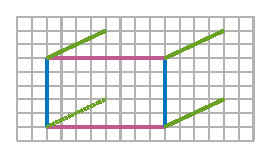
\includegraphics[width=3cm]{persp_rectangle2} \end{center}
  \end{minipage} \hfill%
   \begin{minipage}[c]{0.3\linewidth}   
\begin{center} 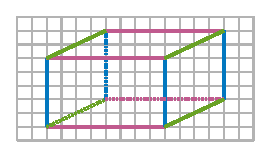
\includegraphics[width=3cm]{persp_rectangle3} \end{center}
   \end{minipage} \\
 \end{exemple*1}

 \begin{exemple*1}
Trace un prisme droit à base triangulaire en perspective cavalière. \\
 \begin{minipage}[c]{0.30\linewidth}
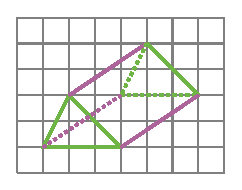
\includegraphics[width=3cm]{persp_triangle} 
  \end{minipage} \hfill%
  \begin{minipage}[c]{0.76\linewidth} 
Les \textcolor{H1}{\textbf{bases}} de ce prisme droit sont des triangles parallèles et superposables. On les représente en vraie grandeur. \\[0.5em]
Les \textcolor{C1}{\textbf{arêtes latérales}} de ce prisme sont parallèles et de même longueur. On les représente par des segments parallèles de même longueur. \\[0.5em]
On trace en pointillés les arêtes cachées. 
   \end{minipage}
 \end{exemple*1}

 \exercice  
Reproduis puis complète les représentations en perspective cavalière ci‑dessous. Les deux premières sont des pavés, la troisième un prisme droit. 
\begin{colenumerate}{3}
 \item
 
 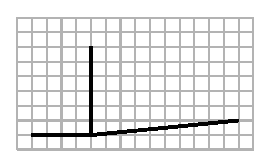
\includegraphics[width=4cm]{persp_ex1} 
 \item
 
 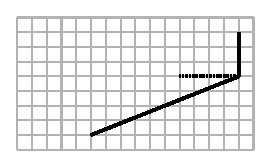
\includegraphics[width=4cm]{persp_ex2} 
 \item 
 
 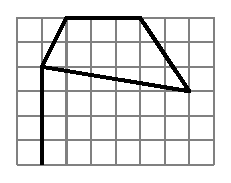
\includegraphics[width=3cm]{persp_ex3}
 \end{colenumerate}
%\correction

% \exercice
 
% \begin{minipage}[c]{0.48\linewidth}
%Reproduis puis complète le tracé en perspective cavalière du prisme droit ci-contre :
%  \end{minipage} \hfill%
%  \begin{minipage}[c]{0.48\linewidth} 
%\begin{center} 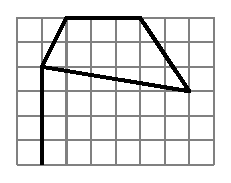
\includegraphics[width=3cm]{persp_ex3} \end{center}
%  \end{minipage} \\
%\correction

 \end{methode*1}
 
 %%%%%%%%%%%%%%%%%%%%%%%%%%%%%%%%%%%%%%%%%%%%%%%%%%%%%%%%%%%%%%%%%%%%%%%%

\begin{methode*1}[Construire un patron]

 \begin{exemple*1}
Construis un patron d'un pavé droit $ABCDEFGH$ tel que $AB = 3$ cm, $AD = 4$ cm et $AE = 5$ cm. 
\begin{center} 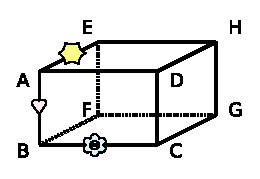
\includegraphics[width=3.5cm]{patron1} \end{center}

 \begin{minipage}[c]{0.75\linewidth}
Un pavé droit comprend trois paires de faces rectangulaires parallèles et de mêmes dimensions.
\begin{itemize}
 \item Les faces ${\textcolor{J1}{ABCD}}$ et $\textcolor{J1}{EFGH}$ mesurent 3 cm par 4 cm ; 
 \item Les faces $\textcolor{C2}{AEHD}$ et $\textcolor{C2}{BFGC}$ mesurent 4 cm par 5 cm ; 
 \item Les faces $\textcolor{H1}{ABFE}$ et $\textcolor{H1}{DCGH}$ mesurent 3 cm par 5 cm.
 \end{itemize}
  \end{minipage} \hfill%
  \begin{minipage}[c]{0.23\linewidth} 
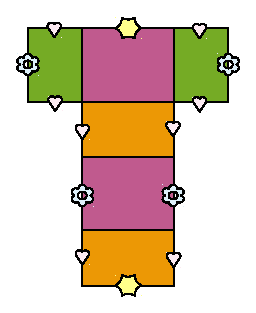
\includegraphics[width=2.5cm]{patron2}  
  \end{minipage} 
Pour obtenir le patron, on peut les disposer « en $T$ ». 
 \end{exemple*1}

 \begin{exemple*1}
Dessine le patron d'un prisme droit dont la base est un triangle de côtés 5 cm, 4 cm et 3 cm, et dont la hauteur est 2 cm.
   
 \begin{minipage}[c]{0.3\linewidth}     
\vspace{-0.2cm}
\begin{center} 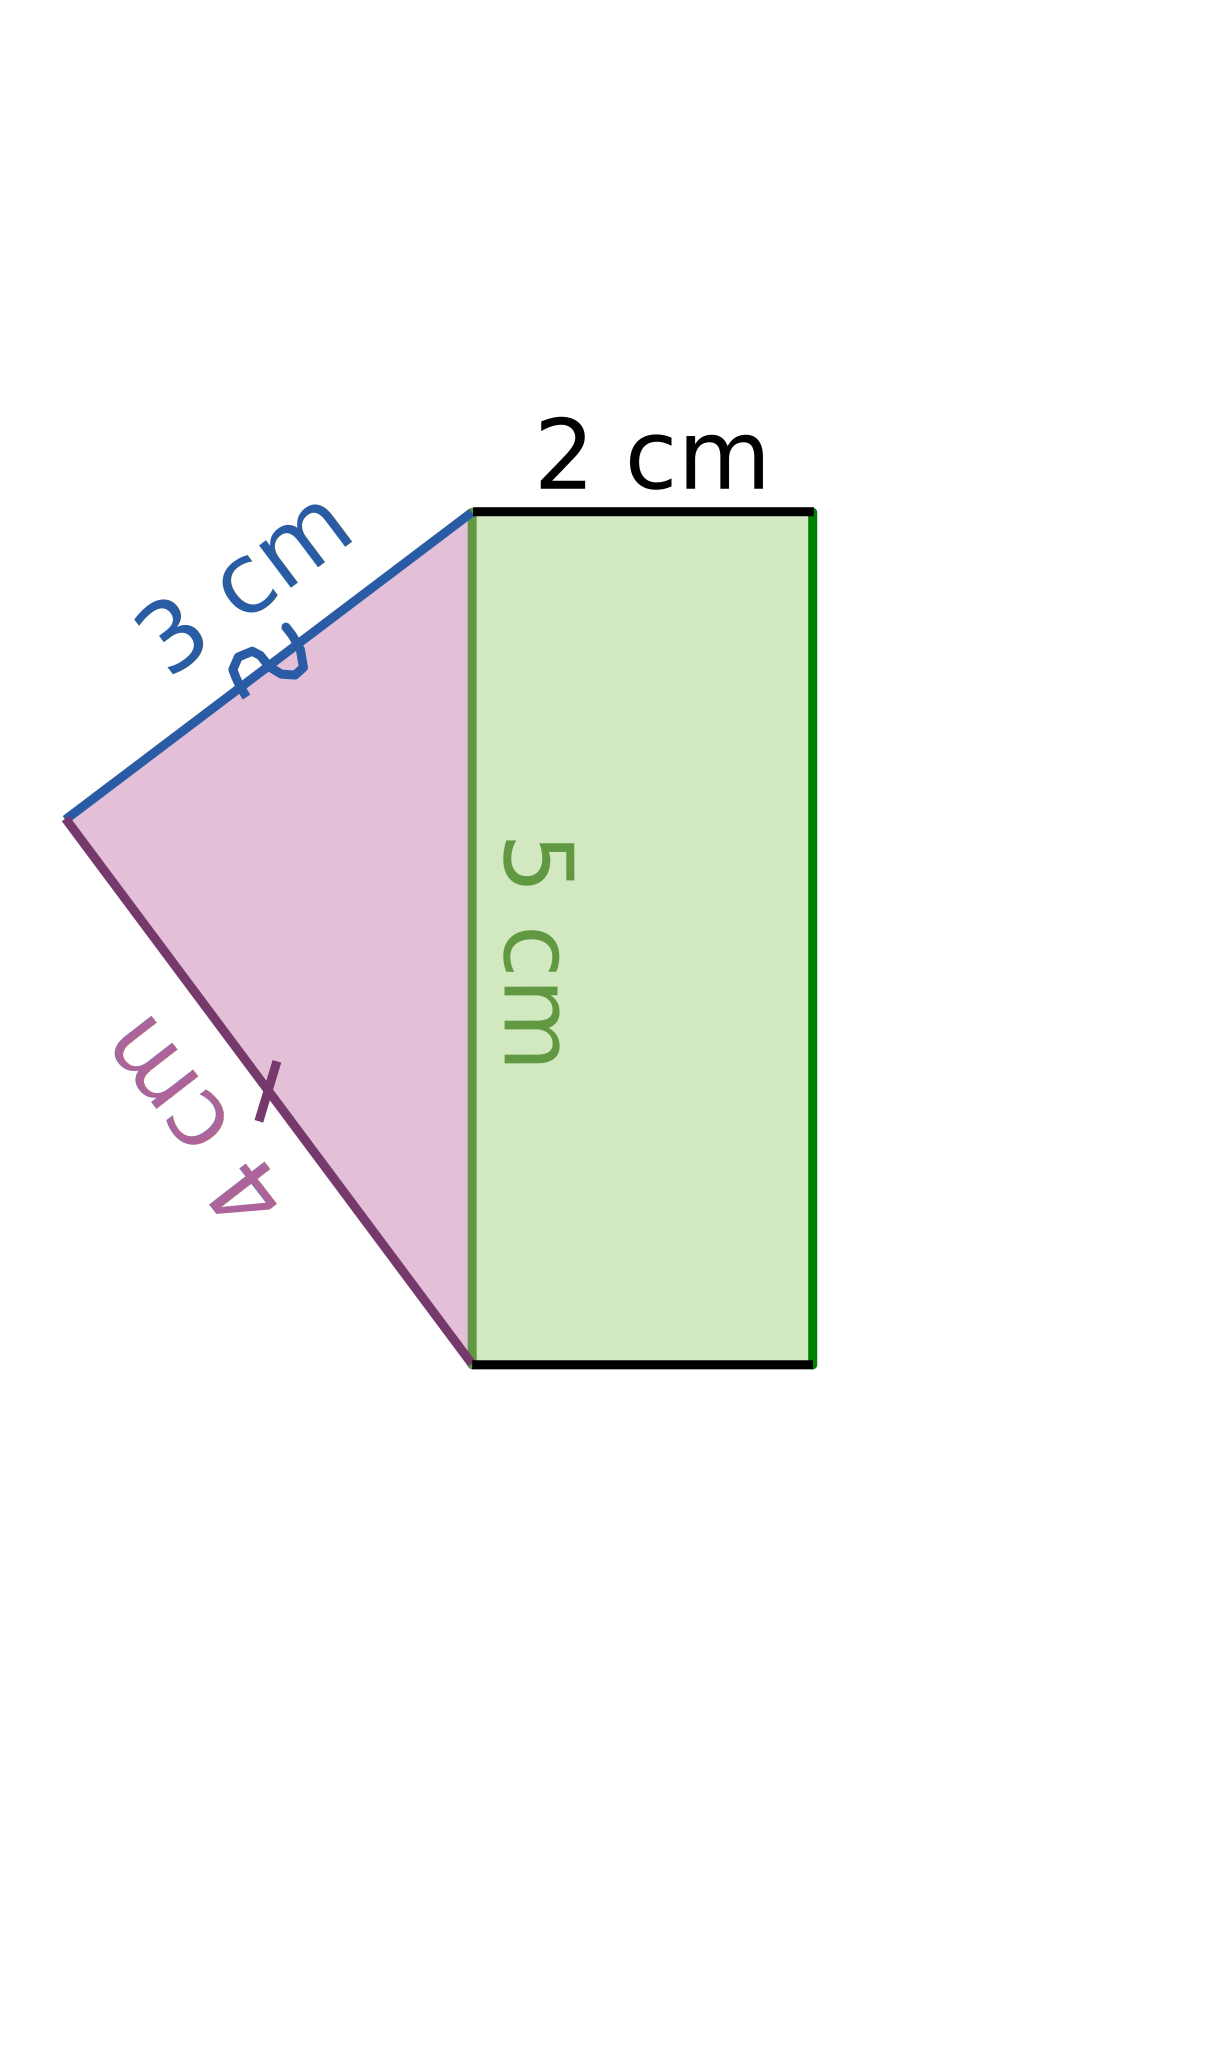
\includegraphics[width=2cm]{patron3} \end{center}
  \end{minipage} \hfill%
  \begin{minipage}[c]{0.3\linewidth}
\begin{center} 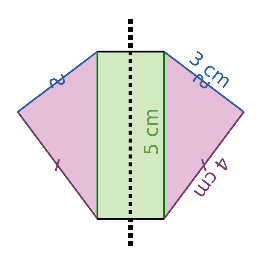
\includegraphics[width=3.1cm]{patron4} \end{center}
  \end{minipage} \hfill%
   \begin{minipage}[c]{0.3\linewidth}   
\begin{center} 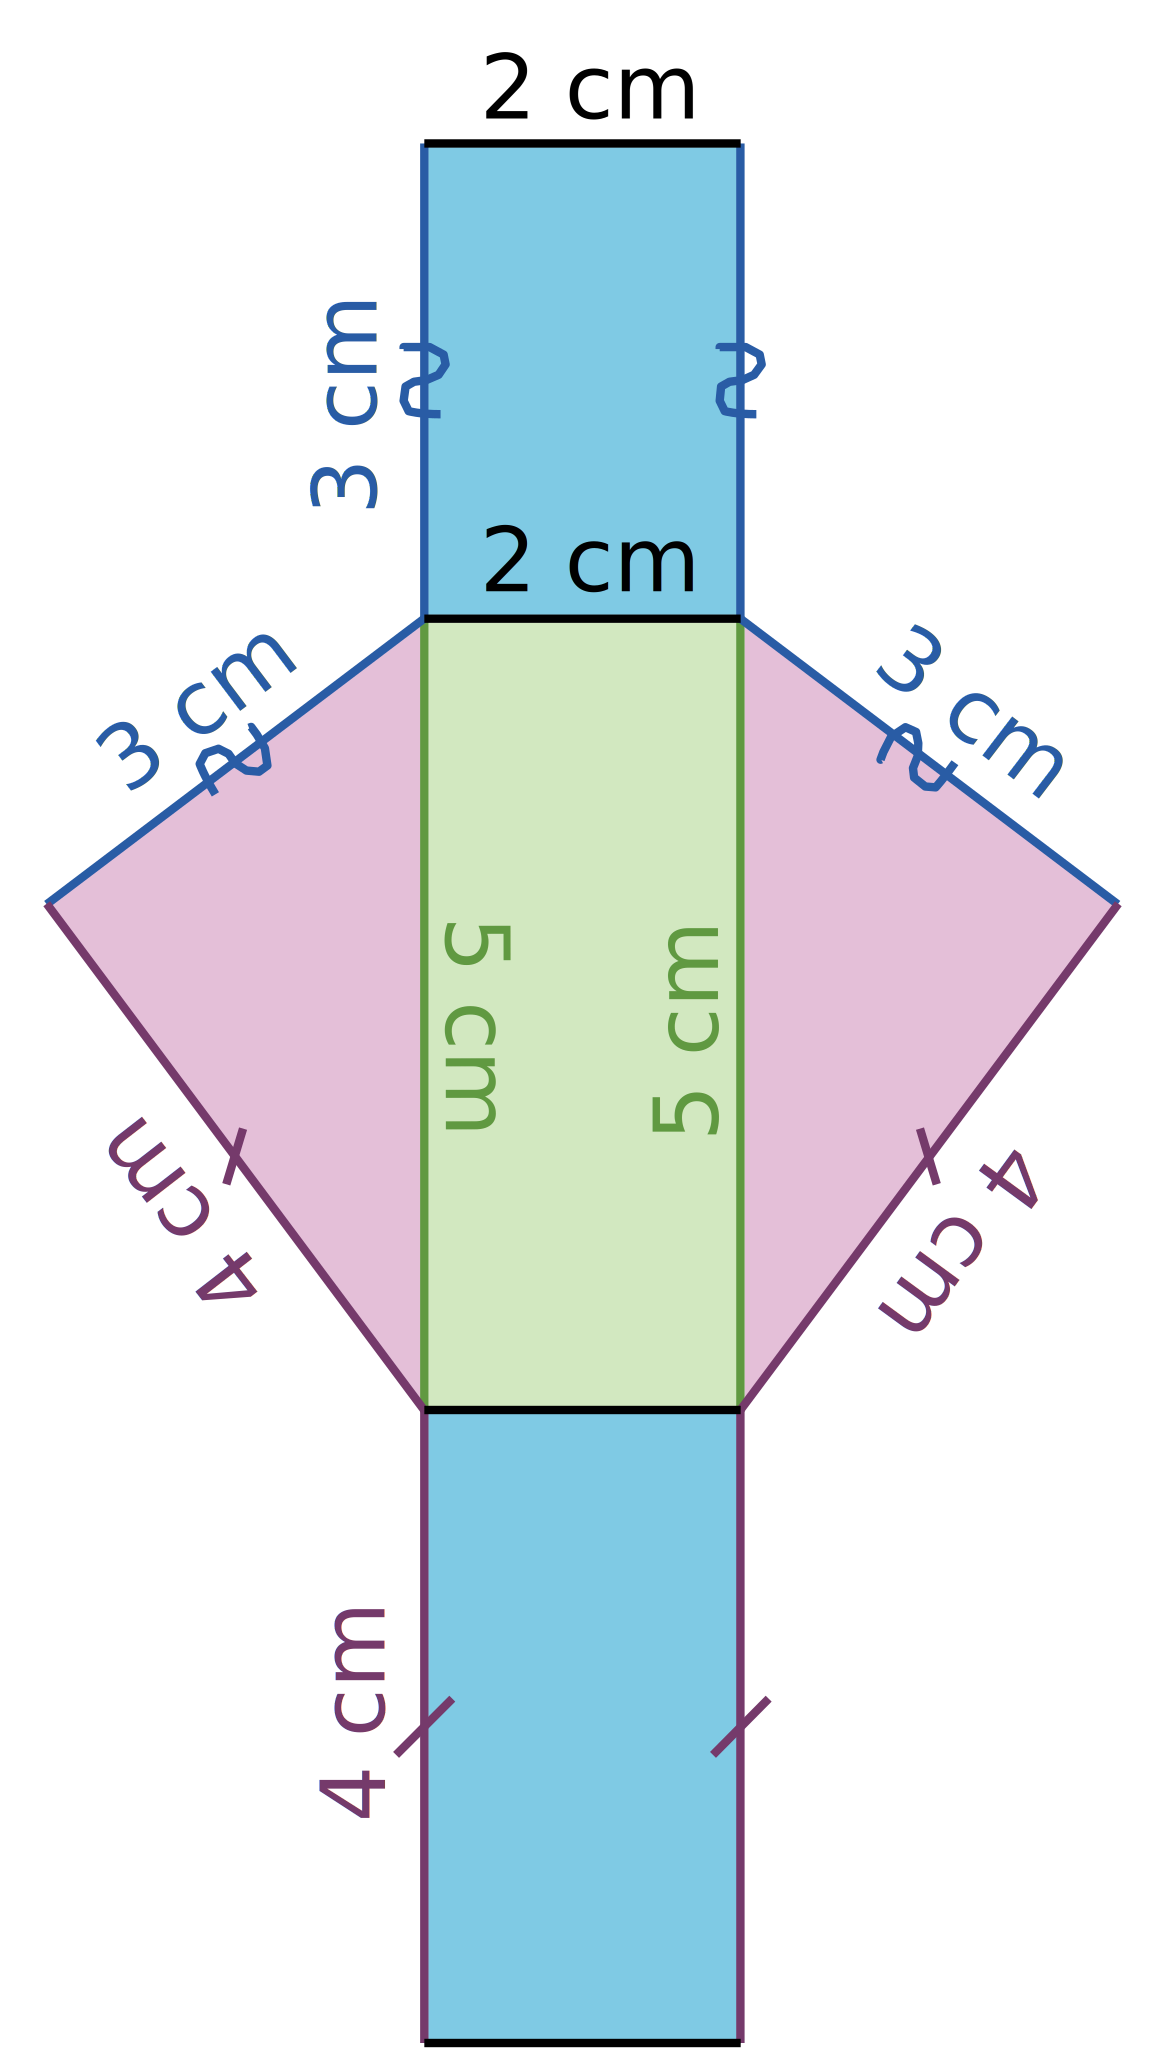
\includegraphics[width=3.2cm]{patron5} \end{center}
   \end{minipage} \\
   
 \begin{minipage}[t]{0.3\linewidth}      
On construit une des \textcolor{C2}{\textbf{bases}}, qui est un triangle, puis on trace une \textcolor{H2}{\textbf{face latérale}} qui est un rectangle dont les côtés sont un côté de la base et la hauteur du prisme droit.
  \end{minipage} \hfill%
  \begin{minipage}[t]{0.3\linewidth}
On trace la seconde \textcolor{C2}{\textbf{base}}, qui est un triangle symétrique au premier par rapport à l'un des axes de symétrie du rectangle.
  \end{minipage} \hfill%
   \begin{minipage}[t]{0.3\linewidth}   
On complète le patron en traçant les deux dernières \textcolor{U1}{\textbf{faces latérales}} du prisme droit, qui sont des rectangles.
   \end{minipage} \\
 \end{exemple*1}

 \exercice  
\begin{enumerate}
\item Construis un patron d'un pavé droit de dimensions 4,5 cm ; 6,2 cm et 3 cm.
\item Construis un patron d'un cube de côté 6,5 cm.
\item Dessine un patron d'un prisme droit de hauteur 3 cm ayant pour base un triangle $ABC$ rectangle en $A$ tel que $AB = 2,5$ cm et $AC = 4$ cm.
\end{enumerate}
%\correction

% \exercice  

%\correction

% \exercice  

%\correction

 \end{methode*1}
 
 %%%%%%%%%%%%%%%%%%%%%%%%%%%%%%%%%%%%%%%%%%%%%%%%%%%%%%%%%%%%%%%%%%%%%%%%
 
 \begin{aconnaitre}
   \begin{minipage}[t]{0.48\linewidth}
  \begin{center} 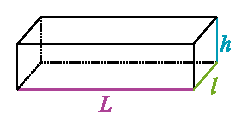
\includegraphics[width=3.8cm]{vol_parall} \end{center}
  \end{minipage} \hfill%
   \begin{minipage}[t]{0.48\linewidth}    
  \begin{center}  
\includegraphics[width=1.5cm]{vol_cube} \end{center}
   \end{minipage} \\
   \begin{minipage}[t]{0.48\linewidth}
  \begin{center} Volume du parallélépipède rectangle \end{center}
  \begin{center} $V = \textcolor{C1}{L} \cdot \textcolor{H1}{l} \cdot \textcolor{U1}{h}$ \end{center}
  \end{minipage} \hfill%
   \begin{minipage}[t]{0.48\linewidth}  
  \begin{center} Volume du cube \end{center}
  \begin{center} $V = \textcolor{J1}{c} \cdot \textcolor{J1}{c} \cdot  \textcolor{J1}{c}$ \end{center}
   \end{minipage} \\[1em]
Les longueurs doivent être exprimées dans la même unité.
\end{aconnaitre}

\begin{methode*1}[Calculer le volume d'un cube et d'un parallélépipède rectangle]

 \begin{remarque}
Un parallélépipède rectangle peut également s'appeler un \textbf{pavé droit}.
 \end{remarque}
 
 \begin{exemple*1}
Calcule le volume d'un pavé droit de 32 mm de longueur, 2,5 cm de largeur et 0,4 dm de hauteur. \\[1em]
\begin{tabular}{lll} 
 $V = \textcolor{C1}{L} \cdot \textcolor{H1}{l} \cdot \textcolor{U1}{h}$ & $\longrightarrow$ & On écrit la formule. \\
 $V = \textcolor{C1}{3,2}\,\text{cm} \cdot \textcolor{H1}{2,5}\,\text{cm} \cdot \textcolor{U1}{4}\,\text{cm}$ ; & $\longrightarrow$ & On remplace par les données \\
 $V = 32\,\text{cm}$\up{3} & & numériques exprimées dans la  \\
 & & même unité : \\
 & & $32\,\text{mm} = 3,2\,\text{cm}$ et $0,4\,\text{dm} = 4\,\text{cm}$. \\
 \end{tabular}
 Le volume du pavé droit est de 32 cm\up{3}.
 \end{exemple*1}


 \exercice  
Calcule le volume d'un cube de 6,1 dm de côté.
%\correction

 \exercice  
\begin{minipage}[c]{0.48\linewidth}
Calcule le volume du solide ci‑contre :
 \end{minipage} \hfill%
 \begin{minipage}[c]{0.28\linewidth}
  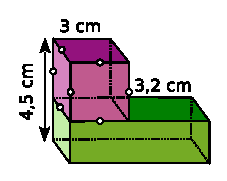
\includegraphics[width=3.4cm]{solide_rosevert}
  \end{minipage} \\
%\correction

 \end{methode*1}
 
 %%%%%%%%%%%%%%%%%%%%%%%%%%%%%%%%%%%%%%%%%%%%%%%%%%%%%%%%%%%%%%%%%%%%%%%%


\exercicesbase
\begin{colonne*exercice}

\serie{Perspective cavalière}

\begin{exercice}[Solides en vrac]
\begin{colenumerate}{2}
 \item
 
 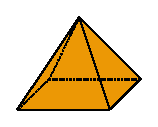
\includegraphics[width=2.3cm]{perspcav_orange}
 \item
 
 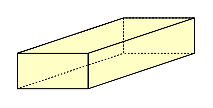
\includegraphics[width=3.2cm]{perspcav_beige}
 \item
 
 
\includegraphics[width=2cm]{perspcav_bleu}
 \item
 
 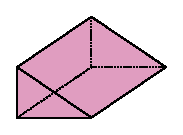
\includegraphics[width=2.7cm]{perspcav_rose}

 \end{colenumerate}
Pour chacun des solides, donne le nombre de sommets, d'arêtes et de faces. 
\end{exercice}


\begin{exercice}[Parallélépipède rectangle] \label{VolSol_entrain2}
Voici la représentation en perspective cavalière d'un parallélépipède rectangle $ABCDEFGH$ :
\begin{center} 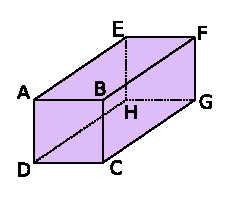
\includegraphics[width=3cm]{parallrect_violet} \end{center}
\begin{enumerate}
 \item Donne deux autres noms possibles pour ce pavé droit.
 \item Combien a‑t‑il de sommets ? Nomme‑les.
 \item Donne le nombre de faces puis nomme‑les.
 \item Combien d'arêtes a‑t‑il ? Nomme‑les.
 \item Nomme les arêtes qui ne sont pas visibles.
 \end{enumerate}
\end{exercice}


\begin{exercice}[Avec un cube] \label{VolSol_entrain1}
Soit le cube $POINTUES$ représenté ci‑dessous :
\begin{center} 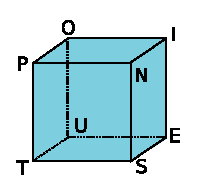
\includegraphics[width=2.6cm]{pointues} \end{center}
\begin{enumerate}
 \item Donne le nombre de sommets, le nombre d'arêtes et le nombre de faces de ce cube.
 \item Quelle est la nature de la face $PNST$ ?
 \item Quelle est la nature de la face $POIN$ ?
 \item Quelles sont les faces cachées du cube ?
 \end{enumerate}
\end{exercice}


\begin{exercice}[Avec un cube (bis)]
La représentation en perspective cavalière du cube $POINTUES$ est à l'exercice \ref{VolSol_entrain1}.
\begin{enumerate}
 \item Nomme la (ou les) face(s) parallèle(s) à la face $POIN$ ;
 \item Nomme la (ou les) face(s) perpendiculaire(s) à la face $PNST$ ;
 \item Cite toutes les arêtes de même longueur que l'arête $[PO]$ ;
 \item Combien d'arêtes ne sont pas visibles ? Nomme‑les ;
 \item Si on pose ce cube sur la face $NIES$, les faces $POIN$ et $OUEI$ étant visibles, quelles sont alors les faces cachées de ce cube ?
 \end{enumerate}
\end{exercice}


\begin{exercice}[Longueurs]
Soit le pavé droit $ABRICOTS$ tel que $AB = 3\,\text{cm}$, $BR = 4\,\text{cm}$ et $AC = 6\,\text{cm}$ :
\begin{enumerate}
 \item Fais, à main levée, une représentation en perspective cavalière de ce pavé droit. Code les arêtes de même longueur sur ton dessin.
 \item Recopie et complète le tableau :
 \begin{center}
  \begin{tabularx}{\linewidth}{|c|*{6}{>{\centering\arraybackslash}X|}}
  \hline
  \cellcolor{C3} Arêtes & \cellcolor{A4} $[IR]$ & \cellcolor{J4} $[BO]$ & \cellcolor{A4} $[CS]$ & \cellcolor{J4} $[RT]$ & \cellcolor{A4} $[CO]$ & \cellcolor{J4} $[OT]$ \\\hline
  \cellcolor{C3} Longueur & \cellcolor{A4} & \cellcolor{J4} & \cellcolor{A4} & \cellcolor{J4} & \cellcolor{A4} & \cellcolor{J4} \\
  \cellcolor{C3} (en cm) & \cellcolor{A4} & \cellcolor{J4} & \cellcolor{A4} & \cellcolor{J4} & \cellcolor{A4} & \cellcolor{J4} \\\hline
  \end{tabularx}
  \end{center}
 \vspace{0.3cm}
 \item Trace en vraie grandeur les faces $ABRI$ et $ABOC$.
 \item En utilisant la figure précédente, donne une valeur approchée de la longueur $BC$.
 \end{enumerate}
\end{exercice}


\begin{exercice}[Vrai / Faux]
On considère le pavé droit de l'exercice \ref{VolSol_entrain2}. Pour chaque affirmation, indique si elle est vraie ou fausse :
\begin{enumerate}
 \item Les faces $ABCD$ et $EFGH$ sont parallèles ;
 \item La face $ABCD$ est un carré ;
 \item L'angle $\widehat{GHD}$ mesure $120^\circ$ environ ;
 \item $ABC$ est un triangle rectangle et isocèle en $B$ ;
 \item L'angle $\widehat{BEF}$ mesure moins de $90^\circ$ ;
 \item L'angle $\widehat{ABF}$ est un angle droit ;
 \item Les arêtes $[AB]$ et $[BF]$ sont parallèles ;
 \item Les arêtes $[EH]$ et $[BF]$ sont sécantes ;
 \item Les arêtes $[CG]$ et $[FG]$ ne sont pas perpendiculaires ;
 \item La face $ADHE$ est un rectangle.
 \end{enumerate}
\end{exercice}


\begin{exercice}[Perspective et pavé droit]
Un parallélépipède rectangle a pour dimensions 2 cm ; 4,5 cm et 5,5 cm :
\begin{enumerate}
 \item Réalise à main levée une représentation possible de ce pavé droit en perspective cavalière puis code ton dessin ;
 \item Construis, à l'aide des instruments de géométrie, une représentation en perspective cavalière de ce pavé droit.
 \end{enumerate}
\end{exercice}


\begin{exercice}[Perspective et cube]
Un cube a une arête de 5 cm :
\begin{enumerate}
 \item À main levée, dessine ce cube en perspective cavalière puis code ton dessin ;
 \item Construis, sur papier quadrillé, une représentation en perspective cavalière de ce cube.
 \end{enumerate}
\end{exercice}


\begin{exercice}
On empile deux cubes identiques d'arête 2 cm l'un sur l'autre :
\begin{enumerate}
 \item Décris le solide obtenu et donne ses dimensions ;
 \item Représente ce solide en perspective cavalière sur papier quadrillé.
 \end{enumerate}
\end{exercice}


\begin{exercice}[Perspective sur quadrillage]
Reproduis puis complète les dessins suivants pour obtenir des représentations en perspective cavalière d'un pavé droit :
\begin{center} 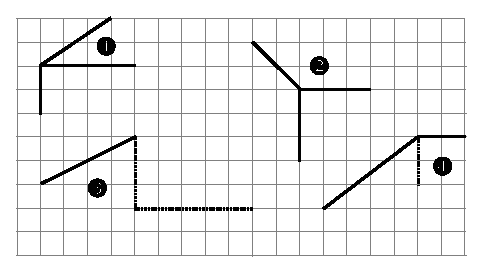
\includegraphics[width=8cm]{persp_quadrillage} \end{center}
\end{exercice}


\begin{exercice}[Araignée]
\begin{minipage}[c]{0.52\linewidth}
Une araignée part du sommet $F$ pour aller au sommet $E$. Elle ne marche que sur les arêtes de ce pavé droit :
 \end{minipage} \hfill%
 \begin{minipage}[c]{0.44\linewidth}
  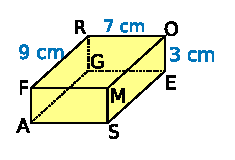
\includegraphics[width=3.5cm]{parcours_araignee}
  \end{minipage} \\
\begin{enumerate}
 \item Quel est le chemin le plus court ? Y a‑t‑il plusieurs possibilités ? Si oui, donne‑les toutes.
 \item Calcule la longueur de ce chemin.
 \end{enumerate}
\end{exercice}


\begin{exercice}[Empilements]
Le solide ci‑dessous est composé de cubes ayant pour arête 3 cm. La face du bas, la face arrière et la face de gauche sont des carrés :
\begin{center} 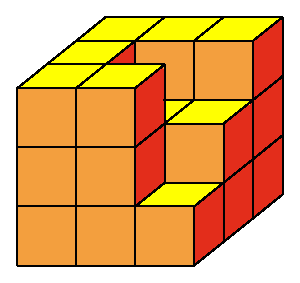
\includegraphics[width=4.7cm]{empilements} \end{center}
\begin{enumerate}
 \item Combien de cubes faudrait‑il ajouter pour obtenir un cube d'arête 9 cm ?
 \item Combien de cubes contient ce solide ?
 \item Dessine en vraie grandeur la face de dessus et la face de droite.
 \end{enumerate}
\end{exercice}


\begin{exercice}[Paquets]
Mandy veut ficeler des paquets de dimensions 20 cm, 15 cm et 50 cm. Elle a besoin de 25 cm par paquet pour faire le nœud. Mandy possède deux pelotes de ficelle de 95 m chacune.
\begin{colenumerate}{2}
 \item
 
 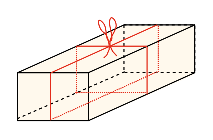
\includegraphics[width=3.1cm]{pelote1} \label{VolSol_entrain3}
 \item
 
 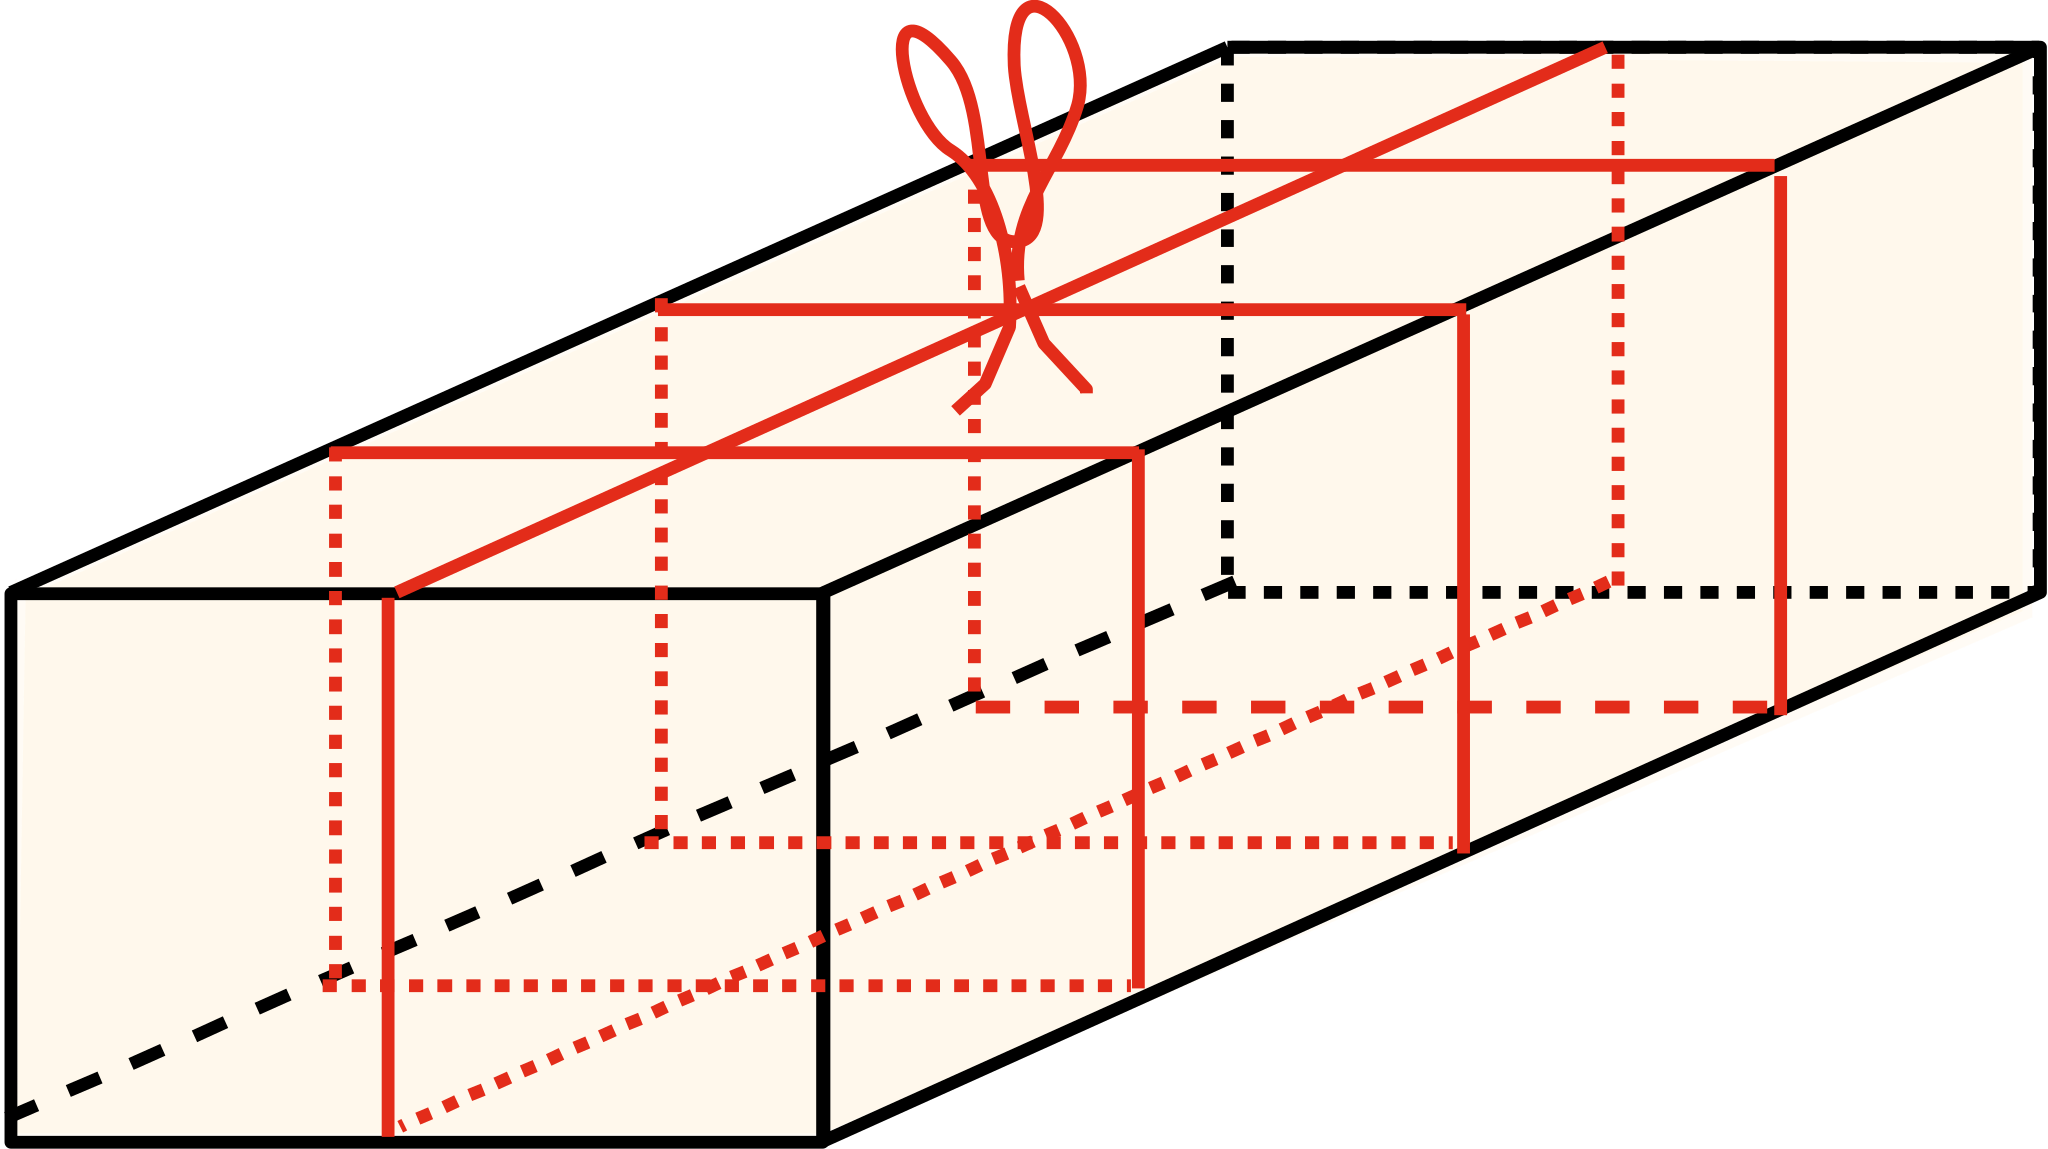
\includegraphics[width=3.1cm]{pelote2} \label{VolSol_entrain4}
 \end{colenumerate}
\begin{itemize}
 \item Pour chaque paquet, donne la longueur en mètres de ficelle utilisée par Mandy.
 \item Combien de paquets \ref{VolSol_entrain3} pourra‑t‑elle ficeler avec une pelote ?
 \item Combien de paquets \ref{VolSol_entrain4} pourra‑t‑elle ficeler avec deux pelotes ?
 \end{itemize}
\end{exercice}


%%%%%%%%%%%%%%%%%%%%%%%%%%%%%%%%%%%
%%%%%%%%%%%%%%%%%%%%%%%%%%%%%%%%%%%
%MiseEnPage
%%%%%%%%%%%%%%%%%%%%%%%%%%%%%%%%%%%
\newpage
%%%%%%%%%%%%%%%%%%%%%%%%%%%%%%%%%%%
%%%%%%%%%%%%%%%%%%%%%%%%%%%%%%%%%%%

%%%%%%%%%%%%%%%%%%%%%%%%%%%%%%%%%%%%%%%%%%%%%%%%%%%%%%%%%%%%%%%%%%%%%%

\serie{Patrons}

\begin{exercice}[Patrons d'un cube ?]
Quels dessins représentent un patron de cube ? 
\begin{colenumerate}{3}
 \item
 
 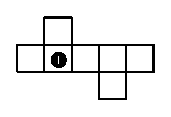
\includegraphics[width=2.4cm]{patron_cube1}
 \item
 
 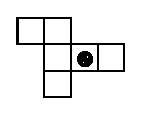
\includegraphics[width=1.9cm]{patron_cube2}
 \item
 
 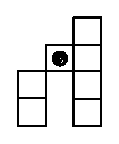
\includegraphics[width=1.5cm]{patron_cube3}
 \item
 
 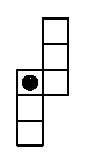
\includegraphics[width=0.9cm]{patron_cube4}
 \item
 
 
\includegraphics[width=1.4cm]{patron_cube5}
 \item
 
 
\includegraphics[width=2.05cm]{patron_cube6}
 \end{colenumerate}
\end{exercice}


\begin{exercice}[Patron et pavé]
Soit une représentation en perspective cavalière et un patron d'un pavé droit :

\begin{minipage}[c]{0.48\linewidth}
 \includegraphics[width=4.3cm]{patron_pave}
 \end{minipage} \hfill%
 \begin{minipage}[c]{0.48\linewidth}
  \includegraphics[width=3.105cm]{patronOM}
  \end{minipage} \\
\begin{enumerate}
 \item Reproduis, à main levée, le patron du pavé droit ; complète le nom des sommets et code les égalités de longueurs. 
 \item Trace ce patron en vraie grandeur.
 \end{enumerate}
\end{exercice}


\begin{exercice}[Patrons d'un pavé ?]
Quels dessins représentent un patron de pavé droit ? Justifie.

\begin{minipage}[c]{0.48\linewidth}
 \includegraphics[width=4.2cm]{patron_pave1}
 \end{minipage} \hfill%
 \begin{minipage}[c]{0.48\linewidth}
  \includegraphics[width=4.1cm]{patron_pave2}
  \end{minipage} \\
\begin{minipage}[c]{0.3\linewidth}
 \includegraphics[width=1.7cm]{patron_pave3}
 \end{minipage} \hfill%
 \begin{minipage}[c]{0.33\linewidth}
  \includegraphics[width=2.5cm]{patron_pave4}
 \end{minipage} \hfill% 
 \begin{minipage}[c]{0.34\linewidth} 
  \includegraphics[width=2.5cm]{patron_pave5}  
  \end{minipage} \\
\end{exercice}


\begin{exercice}[Au choix]
\begin{minipage}[c]{0.68\linewidth}
Associe ce pavé droit à son patron. Justifie.
 \end{minipage} \hfill%
 \begin{minipage}[c]{0.30\linewidth}
  \includegraphics[width=2.1cm]{pave_simple}
  \end{minipage} \\
\begin{minipage}[c]{0.48\linewidth}
  \includegraphics[width=4.1cm]{choix_patron1}
 \end{minipage} \hfill%
 \begin{minipage}[c]{0.44\linewidth}
  \includegraphics[width=3.1cm]{choix_patron2}
  \end{minipage} \\
\end{exercice}


\begin{exercice}
Reproduis, à main levée, chaque patron de pavé droit en complétant les longueurs manquantes :
\begin{minipage}[c]{0.58\linewidth}
  \includegraphics[width=4.7cm]{patron_completer1}
 \end{minipage} \hfill%
 \begin{minipage}[c]{0.38\linewidth}
  \includegraphics[width=2.8cm]{patron_completer2}
  \end{minipage} \\
\end{exercice}

%%%%%%%%%%%%%%%%%%%%%%%%%%%%%%%%%%%
%%%%%%%%%%%%%%%%%%%%%%%%%%%%%%%%%%%
%MiseEnPage
%%%%%%%%%%%%%%%%%%%%%%%%%%%%%%%%%%%
\newpage
%%%%%%%%%%%%%%%%%%%%%%%%%%%%%%%%%%%
%%%%%%%%%%%%%%%%%%%%%%%%%%%%%%%%%%%

\begin{exercice}[Patrons en vrac]
Recopie puis complète chaque patron de pavé droit :
\begin{center} \includegraphics[width=8cm]{patron_pavedroit} \end{center}
\end{exercice}


\begin{exercice}
Trace un patron des solides dont les dimensions sont dans les tableaux ci‑dessous :
\begin{enumerate}
 \item
 
 \begin{center}
  \renewcommand*\tabularxcolumn[1]{>{\centering\arraybackslash}m{#1}}
  \begin{ttableau}{\linewidth}{4}
  \hline
  \rowcolor{C3} Pavé droit & Longueur & Largeur & Hauteur \\\hline
  \cellcolor{C3} \circled{1} & 4,5 cm & 2 cm & 6 cm \\\hline
  \cellcolor{C3} \circled{2} & 27 mm & 1,5 cm & 42 mm \\\hline
  \cellcolor{C3} \circled{3} & 5,3 cm & 25 mm & 74 mm \\\hline
  \end{ttableau}
  \end{center}
 \vspace{0.5cm}
 \item
 
 \begin{center}
  \renewcommand*\tabularxcolumn[1]{>{\centering\arraybackslash}m{#1}}
  \begin{ttableau}{\linewidth}{2}
  \hline
  Cube & Longueur de l'arête \\\hline
  \circled{4} & 4,5 cm \\\hline
  \circled{5} & 56 mm \\\hline
  \end{ttableau}
  \end{center}
 \end{enumerate}
\end{exercice}


\begin{exercice}
\begin{minipage}[c]{0.66\linewidth}
\vspace{1cm}
Réalise un patron de ce cube d'arête 3,6 cm sachant que les motifs sur deux faces opposées sont identiques.
 \end{minipage} \hfill%
 \begin{minipage}[c]{0.28\linewidth}
\vspace{1cm}
  \includegraphics[width=1.7cm]{paquet_rose}
  \end{minipage} \\
\end{exercice}


\begin{exercice}
\begin{minipage}[c]{0.46\linewidth}
\vspace{1.9cm}
Réalise un patron de ce pavé droit composé de trois cubes identiques d'arête 2 cm, en respectant les couleurs.
 \end{minipage} \hfill%
 \begin{minipage}[c]{0.46\linewidth}
 \vspace{1cm}
  \includegraphics[width=3.4cm]{3cubes_colores}
  \end{minipage} \\
\end{exercice}


%%%%%%%%%%%%%%%%%%%%%%%%%%%%%%%%%%%
%%%%%%%%%%%%%%%%%%%%%%%%%%%%%%%%%%%
%MiseEnPage
%%%%%%%%%%%%%%%%%%%%%%%%%%%%%%%%%%%
\columnbreak
%%%%%%%%%%%%%%%%%%%%%%%%%%%%%%%%%%%
%%%%%%%%%%%%%%%%%%%%%%%%%%%%%%%%%%%

%%%%%%%%%%%%%%%%%%%%%%%%%%%%%%%%%%%%%%%%%%%%%%%%%%%%%%%%%%%%%%%%%%%%%%

\serie{Calculer des volumes}

\begin{exercice}[Volume par comptage]
\includegraphics[width=0.7cm]{unite_volume} est 1 unité de volume.

 Donne le volume de chaque solide en unités de volume. Les volumes sont supposés pleins.
\begin{colenumerate}{2}
 \item
 
 \includegraphics[width=3.4cm]{unite_volA} 
 
 \item
 
 \includegraphics[width=2.2cm]{unite_volB} 
 
 \item
 
 \includegraphics[width=1.8cm]{unite_volC} 
 
 \item
 
 \includegraphics[width=3.7cm]{unite_volD} 
 
 \item
 
 \includegraphics[width=1.8cm]{unite_volE} 
 \end{colenumerate}
\end{exercice}


\begin{exercice}[Volume de pavés]
Recopie le tableau et calcule les valeurs de $a$, $b$, $c$, $d$, $e$ et $f$ :
\begin{center}
 \begin{tabularx}{\linewidth}{|c|*{4}{>{\centering\arraybackslash}X|}}
 \hline
 & \cellcolor{H2} Longueur & \cellcolor{H2} Largeur & \cellcolor{H2} Hauteur & \cellcolor{H2} Volume \\\hline
 \cellcolor{U1} $P_1$ & \cellcolor{H3} 3 cm & \cellcolor{H3} 1 cm & \cellcolor{H3} 2 cm & \cellcolor{H3} $a$ \\\hline
 \cellcolor{U1} $P_2$ & \cellcolor{H3} 3,5 mm & \cellcolor{H3} 2 mm & \cellcolor{H3} 1 mm & \cellcolor{H3} $b$ \\\hline
 \cellcolor{U1} $P_3$ & \cellcolor{H3} 2,2 dm & \cellcolor{H3} 8 cm & \cellcolor{H3} 3 dm & \cellcolor{H3} $c$ \\\hline
 \cellcolor{U1} $P_4$ & \cellcolor{H3} 6 dm & \cellcolor{H3} 5 dm & \cellcolor{H3} $d$ & \cellcolor{H3} 120 dm\up{3} \\\hline
 \cellcolor{U1} $P_5$ & \cellcolor{H3} $e$ & \cellcolor{H3} 4 m & \cellcolor{H3} 3,2 m & \cellcolor{H3} 74,24 m\up{3} \\\hline
 \cellcolor{U1} $P_6$ & \cellcolor{H3} 2,5 hm & \cellcolor{H3} 2,7 dam & \cellcolor{H3} $f$ & \cellcolor{H3} 81 dam\up{3} \\\hline
 \end{tabularx}
 \end{center}
\end{exercice}

%%%%%%%%%%%%%%%%%%%%%%%%%%%%%%%%%%%
%%%%%%%%%%%%%%%%%%%%%%%%%%%%%%%%%%%
%MiseEnPage
%%%%%%%%%%%%%%%%%%%%%%%%%%%%%%%%%%%
\newpage
%%%%%%%%%%%%%%%%%%%%%%%%%%%%%%%%%%%
%%%%%%%%%%%%%%%%%%%%%%%%%%%%%%%%%%%

\begin{exercice}[Des solides]
Calcule le volume de chaque solide constitués de parallélépipèdes rectangles :
\begin{colenumerate}{2}
 \item 
 
 \includegraphics[width=3.8cm]{croix_rose}
 \item 
 
 \includegraphics[width=5.5cm]{marche_orange}
 \item 
 
 \includegraphics[width=2.5cm]{pile_verte}

 \end{colenumerate}
\end{exercice}


\begin{exercice}[Attention aux unités]
\begin{enumerate}
 \item Un cube de côté 1,2 m est percé de part en part par un trou fait à partir d'un carré de côté 12 cm. Calcule le volume du solide obtenu : \\[0.3em]
 \begin{center} \includegraphics[width=3.2cm]{double_cube} \end{center}
 \item Calcule en cm\up{3} le volume de ce solide : \\[0.3em]
 \begin{center} \includegraphics[width=5cm]{3marches} \end{center}
 \end{enumerate}
\end{exercice}


\begin{exercice}[Des tables]
Une table est composée d'un plateau rectangulaire de 3 cm d'épaisseur qui mesure 1,3 m de long et 0,8 m de large. Les pieds ont une base carrée de 9 cm de côté et une hauteur de 72 cm. \\[0.3em]
 \begin{center} \includegraphics[width=5cm]{table_brune} \end{center}
 \begin{enumerate}
  \item Calcule le volume de bois nécessaire pour fabriquer cette table.
  \item Le chêne qui constitue cette table a une densité d'environ 0,7, ce qui signifie qu'un mètre cube de chêne pèse 700 kg. Combien pèse cette table si on la construit en chêne ?
  \item Une autre table construite en ébène (densité = 1,10) a une masse de 60,5 kg. Quel est le volume de cette table ?
  \end{enumerate}
\end{exercice}


\end{colonne*exercice}


\exercicesappr
\begin{colonne*exercice}
\begin{exercice}[Visible ou caché ?]
\begin{minipage}[c]{0.48\linewidth}
La figure ci‑contre représente les huit sommets d'un pavé droit. Reproduis deux   figures similaires puis complète‑les de façon à ce que les quatre points marqués en rouge forment :
 \end{minipage} \hfill%
 \begin{minipage}[c]{0.48\linewidth}
  \includegraphics[width=3.5cm]{figures_cachees}
  \end{minipage} \\
\begin{enumerate}
 \item La face de devant sur la première figure ;
 \item La face de derrière sur la deuxième figure.
 \end{enumerate}
\end{exercice}


\begin{exercice}[Triangles particuliers]
\begin{minipage}[c]{0.38\linewidth}
On a représenté ci-contre un cube d'arête 4,5 cm.
 \end{minipage} \hfill%
 \begin{minipage}[c]{0.58\linewidth}
  \includegraphics[width=2.5cm]{triangleBFG}
  \end{minipage} \\
\begin{enumerate}
 \item Quelle est dans la réalité la nature du triangle $BFG$ ? Justifie.
 \item Quelle est dans la réalité la nature du triangle $GBD$ ? Justifie.
 \item Construis ces deux triangles en vraie grandeur.
 \end{enumerate}
\end{exercice}


\begin{exercice}[Triangles particuliers (bis)] \label{VolSol_approf1}
$ABRINEUF$ est un pavé droit représenté ci‑après en perspective cavalière. On donne $BR = 7 \text{cm}$ et $AN = AB = 4 \text{cm}$.
 \begin{center} \includegraphics[width=4cm]{abrineuf} \end{center}
 \begin{enumerate}
  \item Quelle est dans la réalité la nature :
  \begin{itemize}
   \item du triangle $ABI$ ?
   \item du triangle $BIN$ ?
    \end{itemize}
Justifie tes réponses.
 \item Construis ces deux triangles en vraie grandeur.
 \end{enumerate}
\end{exercice}


\begin{exercice}[Se méfier des apparences]
On considère le parallélépipède rectangle de l'exercice \ref{VolSol_approf1}.
\begin{enumerate}
 \item Nomme deux arêtes qui sont perpendiculaires dans la réalité, mais pas sur le dessin.
 \item Peux‑tu répondre à la même question en remplaçant le mot « perpendiculaires » par « parallèles » ?
 \end{enumerate}
\end{exercice}


\begin{exercice}[Vrai ou faux ?]
On considère le parallélépipède rectangle de l'exercice \ref{VolSol_approf1}.
\begin{enumerate}
 \item Que peux-tu dire :
 \begin{itemize}
  \item des droites $(AN)$ et $(AI)$ ?
  \item des droites $(AB)$ et $(AI)$ ?
  \end{itemize}
 \item Que penses‑tu alors de l'affirmation : « Si deux droites sont perpendiculaires à une même droite alors elles sont parallèles. » ?
 \end{enumerate}
\end{exercice}


\begin{exercice}[Belle perspective]
\begin{minipage}[c]{0.44\linewidth} 
\includegraphics[width=3.2cm]{motif_persp}
 \end{minipage} \hfill%
 \begin{minipage}[c]{0.52\linewidth}
\begin{enumerate}
 \item Reproduis le cube ci‑contre en perspective cavalière sur papier quadrillé.
 \item Reproduis sur chaque face visible le motif figurant sur la face de devant.
 \end{enumerate}
  \end{minipage} \\
\end{exercice}


\begin{exercice}[La bonne marche à suivre]
\begin{minipage}[c]{0.52\linewidth} 
En collant des blocs cubiques identiques de 40 cm d'arête, on a construit un escalier comprenant quatre marches. Cet escalier doit ensuite être verni.
 \end{minipage} \hfill%
 \begin{minipage}[c]{0.44\linewidth}
 \includegraphics[width=3.2cm]{suivre_marche}
  \end{minipage} \\
\begin{enumerate}
 \item Combien de cubes constituent l'escalier ?
 \item Combien de faces carrées vont être vernies, sachant qu'on ne vernit pas la partie en contact avec le sol ou avec le mur ?
 \item Un pot de 1 L de vernis couvre 15 m\up{2}. Combien faudra‑t‑il de pots pour passer deux couches sur l'escalier ? 
 \item Calcule le nombre de cubes nécessaires à la fabrication d'un escalier semblable mais comprenant 100 marches.
 \end{enumerate}
\end{exercice}

%%%%%%%%%%%%%%%%%%%%%%%%%%%%%%%%%%%
%%%%%%%%%%%%%%%%%%%%%%%%%%%%%%%%%%%
%MiseEnPage
%%%%%%%%%%%%%%%%%%%%%%%%%%%%%%%%%%%
\newpage
%%%%%%%%%%%%%%%%%%%%%%%%%%%%%%%%%%%
%%%%%%%%%%%%%%%%%%%%%%%%%%%%%%%%%%%

\begin{exercice}[Des dés]
\begin{minipage}[c]{0.78\linewidth} 
Sur un dé à jouer, la somme des nombres de points inscrits sur deux faces opposées est égale à 7.
 \end{minipage} \hfill%
 \begin{minipage}[c]{0.18\linewidth}
 \includegraphics[width=1.5cm]{des1}
  \end{minipage} \\
\begin{minipage}[c]{0.78\linewidth} 
\begin{enumerate}
 \item Construis un patron du dé ci‑dessus puis marque les points sur chaque face.
 \item Sachant que le dé est à présent posé sur la face à trois points, combien de points comporte la face du dessus ? Et la face de droite ?
 \end{enumerate}
 \end{minipage} \hfill%
 \begin{minipage}[c]{0.18\linewidth}
 \includegraphics[width=1.5cm]{des2}
  \end{minipage} \\
\end{exercice}


\begin{exercice}[Patron]
On donne ci‑dessous la vue de face et la vue de côté d'un solide composé de deux parallélépipèdes rectangles accolés :
\begin{enumerate}
 \item Donne les dimensions de chaque parallélépipède rectangle.
 \item Fais un patron de chacun d'entre eux.
 \end{enumerate}
\begin{center} \includegraphics[width=8cm]{dim_patron} \end{center}
\end{exercice}


\begin{exercice}[Un solide peut en cacher un autre]
On considère un cube de 5 cm d'arête :
\begin{enumerate}
 \item Sur papier quadrillé, trace une représentation en perspective cavalière de ce cube puis marque les milieux des arêtes de la face de « dessus » et de la face de « dessous ».
 \item Décris le solide obtenu en reliant les huit points que tu as marqués. Fais‑en un patron.
 \item Que se passe‑t‑il si on recommence le processus ?
 \end{enumerate}
 \begin{center} \includegraphics[width=5cm]{cube_cacher} \end{center}
\end{exercice}


\begin{exercice}[Chasse d'eau]
Un réservoir de chasse d'eau a la forme d'un pavé droit de 30 cm de longueur, 24 cm de largeur et 18 cm de hauteur. Il est rempli aux trois quarts de sa hauteur. Combien de litres d'eau sont utilisés lorsqu'on tire cette chasse d'eau ?
\end{exercice}


\begin{exercice}[Cube percé]
Calcule le volume de ce solide qui est un cube percé de part en part au centre de chaque face :
 \begin{center} \includegraphics[width=4.5cm]{cube_perce} \end{center}
\end{exercice}


\begin{exercice}[Des pièces]
Les figures ci‑dessous représentent deux pièces d'un jeu. Compare leurs volumes respectifs :
 \begin{center} \includegraphics[width=4.5cm]{pieces_jeu1} \end{center}
 
 \begin{center} \includegraphics[width=4.5cm]{pieces_jeu2} \end{center}
\end{exercice}




\end{colonne*exercice}

\connaissances

\QCMautoevaluation{Pour chaque question, plusieurs réponses sont
  proposées.  Déterminer celles qui sont correctes.}

\begin{QCM}
  \begin{GroupeQCM}
  
      \begin{center} \includegraphics[width=4.5cm]{paveABCDEFGH} \end{center}
      \begin{center} $ABCDEFGH$ est un pavé droit. \end{center}
      
    \begin{exercice}
      \begin{ChoixQCM}{4}
      \item $[HD]$ est une arête
      \item $[EF]$ est une arête
      \item $[BG]$ est une arête
      \item $[AG]$ est une arête
      \end{ChoixQCM}
\begin{corrige}
     \reponseQCM{ab}
   \end{corrige}
    \end{exercice}
    
    \begin{exercice}
      \begin{ChoixQCM}{4}
      \item La longueur $EA$  sur la figure est en vraie grandeur
      \item La longueur $FG$  sur la figure est en vraie grandeur
      \item La longueur $FC$  sur la figure est en vraie grandeur
      \item La longueur $HC$  sur la figure est en vraie grandeur
      \end{ChoixQCM}
\begin{corrige}
     \reponseQCM{ad}
   \end{corrige}
    \end{exercice}
    
    
     \begin{exercice}
      \begin{ChoixQCM}{4}
      \item Les faces $ABCD$ et $AEFB$ sont parallèles
      \item Les faces $ABCD$ et $EFGH$ sont parallèles
      \item Les faces $EADH$ et $FBCG$ sont parallèles
      \item Les faces $EADH$ et $EFGH$ sont parallèles
      \end{ChoixQCM}
\begin{corrige}
     \reponseQCM{bc}
   \end{corrige}
    \end{exercice}
    
    
     \begin{exercice}
      \begin{ChoixQCM}{4}
      \item $AB = EF = HG$
      \item $FG = EF$
      \item $EH = AD = HG$
      \item $HD = EA = FB$
      \end{ChoixQCM}
\begin{corrige}
     \reponseQCM{ad}
   \end{corrige}
    \end{exercice}
    
    
     \begin{exercice}
      \begin{ChoixQCM}{4}
      \item $(AD)$ est perpendiculaire à $(AB)$
      \item $(AD)$ et $(BC)$ sont parallèles
      \item $(AD)$ et $(DC)$ sont parallèles
      \item $(AD)$ est perpendiculaire à $(HD)$
      \end{ChoixQCM}
\begin{corrige}
     \reponseQCM{abd}
   \end{corrige}
    \end{exercice}
    
    
     \begin{exercice}
      \begin{ChoixQCM}{4}
      \item $FBC$ est équilatéral
      \item $FHE$ est isocèle en $F$
      \item $BCD$ est quelconque
      \item $FBC$ est rectangle en $B$
      \end{ChoixQCM}
\begin{corrige}
     \reponseQCM{d}
   \end{corrige}
    \end{exercice}

    
    \begin{exercice}
      Le pavé ABCDEFGH a pour patron(s) possible(s) \ldots
      \begin{ChoixQCM}{4}
      \item \includegraphics[width=2cm]{ABCDEFGH_patron1}
      \item \includegraphics[width=2cm]{ABCDEFGH_patron2}
      \item \includegraphics[width=2cm]{ABCDEFGH_patron3}
      \item \includegraphics[width=2cm]{ABCDEFGH_patron4}
      \end{ChoixQCM}
\begin{corrige}
     \reponseQCM{abd}
   \end{corrige}
    \end{exercice}
 \end{GroupeQCM}
\end{QCM}   
    
    
\begin{QCM}
  \begin{GroupeQCM}
      
    \begin{exercice}
      Le volume d'un cube de 3 cm d'arête est \ldots
      \begin{ChoixQCM}{4}
      \item 3 cm\up{3}
      \item 9 cm\up{3}
      \item 27 cm\up{3}
      \item 12 cm\up{3}
      \end{ChoixQCM}
\begin{corrige}
     \reponseQCM{c}
   \end{corrige}
    \end{exercice}


    \begin{exercice}
      Quelle phrase est vraie ?
      \begin{ChoixQCM}{4}
      \item Si on double la longueur de l'arête d'un cube alors son volume double aussi
      \item Si on double la longueur de l'arête d'un cube alors son volume est multiplié par 4
      \item Si on double la longueur de l'arête d'un cube alors son volume est multiplié par 8
      \item Si on double la longueur de l'arête d'un cube alors son volume est multiplié par 16
      \end{ChoixQCM}
\begin{corrige}
     \reponseQCM{c}
   \end{corrige}
    \end{exercice}
    
    
    \begin{exercice}
      Mon volume est de 12 cm\up{3} et la longueur totale de mes arêtes est de 28 cm. Qui puis‑je être ?
      \begin{ChoixQCM}{4}
      \item Je suis un pavé de dimensions  2 ; 2 et 3 en centimètres
      \item Je suis un cube d'arête 3 cm
      \item Je suis un pavé de dimensions 2 ; 7 et 2 en centimètres
      \item Je suis un pavé de dimensions  6 ; 2 et 1 en centimètres
      \end{ChoixQCM}
\begin{corrige}
     \reponseQCM{a}
   \end{corrige}
    \end{exercice}


\end{GroupeQCM}
\end{QCM}

  


\TravauxPratiques % pour nous "travailler en groupe"

\begin{TP}[Eponge de Menger]

\partie{Réalisation}

\begin{enumerate}
 \item Réalisez 20 cubes identiques en papier d'arêtes 4 cm.
 \item Placez ces 20 copies de telle façon qu'elles forment un nouveau cube de 12 cm d'arêtes  sans les parties centrales. Comme le dessin ci-dessous :
 \begin{center} \includegraphics[width=2.8cm]{menger1} \end{center}
 \begin{center} Étape 1 \end{center}
 \item Regroupez toutes les copies des cubes réalisées et complétez leurs nombres pour en avoir 400. Placez ces 400 copies de telle façon qu'elles forment un nouveau cube de 36 cm d'arêtes  sans les parties centrales. Comme le dessin ci-dessous :
 \begin{center} \includegraphics[width=2.8cm]{menger2} \end{center}
 \begin{center} Étape 2 \end{center}
 \item Combien de cubes seraient nécessaire pour construire la 3\up{ème} étape ? Quelle hauteur atteindrait l'éponge de Menger ?
 \begin{center} \includegraphics[width=6cm]{menger3} \end{center}
 \qquad \qquad \qquad \qquad \qquad \qquad \qquad \qquad \qquad \qquad \small{\emph{(Wikipedia, auteur : Solkoll)}}
 \end{enumerate}

\partie{Volumes}

La construction d'une éponge de Menger peut être décrite de la manière suivante :
\begin{itemize}
 \item Débuter par un cube ;
 \item Réduire le cube au tiers et en faire 20 copies ;
 \item Placer ces copies de telle façon qu'elles forment un nouveau cube de la même taille que l'original, sans les parties centrales ;
 \item Répéter le processus à partir de l'étape 2 pour chacun des 20 cubes ainsi créés.
 \end{itemize} 
Le solide obtenu à la limite, après un nombre infini d'itérations, est l'éponge de Menger.
\begin{enumerate}
 \setcounter{enumi}{4}
 \item Que vaut le volume de l'étape 0, si on prend un cube d'arête 9 cm ?
 \item Que vaut le volume de l'étape 1 ? l'étape 2 ? et l'étape 3 ?
 \item Que dire du volume à l'étape 10 ? et 100 ?
 \item Que peut-on conclure ?
 \end{enumerate}
Ci-dessous, une éponge de Menger, coupée par un plan transversal passant par les milieux des six côtés du cube.
 \begin{center} \includegraphics[width=6cm]{menger4} \end{center}
 \qquad \qquad \qquad \qquad \qquad \qquad \qquad \qquad \qquad \qquad \small{\emph{(Wikipedia, auteur : Theon)}}
 
\end{TP}



\pagebreak

\recreation
\begin{enigme}[Un petit jeu de construction]

\begin{minipage}[c]{0.58\linewidth}
Comme cadeau de Noël, Zohra a eu un jeu avec des petites tiges aimantées et des boules métalliques. Au bout de chaque tige, on peut aimanter une autre tige ou une boule.
 \end{minipage} \hfill%
 \begin{minipage}[c]{0.38\linewidth}
  \includegraphics[width=5cm]{allumettes}
  \end{minipage} \\
Elle dispose de 48 tiges et de 8 boules. Elle cherche à construire, en utilisant tout ce matériel, le pavé droit le plus volumineux possible.
\begin{enumerate}
 \item Quels pavés droits peut‑elle construire ?
 \item Quel est celui qui a le plus grand volume ? Le plus petit volume ?
 \end{enumerate}

\end{enigme} 



